%=======================================================================
%  Academic presentation — Brain Tumor MRI Classification (ML)
%  Compile:  .\build.ps1
%=======================================================================
\documentclass[aspectratio=169,11pt]{beamer}

% Beamer preamble — academic ML presentation (English)
\usepackage[T1]{fontenc}
\usepackage[utf8]{inputenc}
\usepackage[english]{babel}
\usepackage{amsmath,amssymb}
\usepackage{graphicx}
\usepackage{grffile}
\usepackage{booktabs}
\usepackage{array}
\usepackage{multirow}
\usepackage{tikz}
\usetikzlibrary{arrows.meta, positioning, shapes.geometric, fit, calc}
\usepackage{siunitx}
\usepackage{csquotes}
\usepackage[backend=biber,style=ieee,maxbibnames=2,minbibnames=1]{biblatex}
\addbibresource{references.bib}

\IfFileExists{beamerthememetropolis.sty}{%
  \usetheme{metropolis}%
  \usepackage{appendixnumberbeamer}%
}{%
  \usetheme{Madrid}%
}
\usecolortheme{default}

\definecolor{accent}{HTML}{2E5A88}
\definecolor{accent2}{HTML}{1F6F54}
\definecolor{greytx}{HTML}{555555}
\definecolor{lightbg}{HTML}{EAF1F8}

\setbeamercolor{structure}{fg=accent}
\setbeamercolor{frametitle}{fg=white,bg=accent}
\setbeamercolor{title}{fg=white,bg=accent}
\setbeamercolor{block title}{bg=accent!18,fg=accent}
\setbeamercolor{block body}{bg=accent!6}
\setbeamercolor{alerted text}{fg=accent2}

\setbeamertemplate{navigation symbols}{}
\setbeamertemplate{footline}{%
  \leavevmode%
  \hbox{%
    \begin{beamercolorbox}[wd=.45\paperwidth,ht=2.4ex,dp=1ex,leftskip=1em]{author in head/foot}%
      \usebeamerfont{author in head/foot}\insertshortauthor
    \end{beamercolorbox}%
    \begin{beamercolorbox}[wd=.45\paperwidth,ht=2.4ex,dp=1ex,center]{title in head/foot}%
      \usebeamerfont{title in head/foot}\insertshorttitle
    \end{beamercolorbox}%
    \begin{beamercolorbox}[wd=.1\paperwidth,ht=2.4ex,dp=1ex,rightskip=1em]{date in head/foot}%
      \usebeamerfont{date in head/foot}\insertframenumber/\inserttotalframenumber
    \end{beamercolorbox}%
  }%
}

\graphicspath{
  {../../output/}
  {../../PAPER/latex/figures/}
}

\newcommand{\timing}[1]{\textcolor{greytx}{\footnotesize #1}}
\newcommand{\keyresult}[1]{\textcolor{accent2}{\textbf{#1}}}
\newcommand{\interp}[1]{%
  \vspace{0.3em}%
  \begin{block}{Interpretation}%
    \small #1%
  \end{block}%
}

% \setbeameroption{show notes on second screen=right}

%=======================================================================
%  metrics.tex — single source of truth for presentation numbers
%=======================================================================

% --- Dataset ---
\newcommand{\NClasses}{3}
\newcommand{\NTotal}{1\,500}
\newcommand{\NPerClass}{500}
\newcommand{\NTrain}{1\,200}
\newcommand{\NTest}{300}
\newcommand{\NTestPerClass}{100}
\newcommand{\ImgSize}{$128\times128$}

% --- Phase 1 best parameters ---
\newcommand{\statsParams}{11 first-order intensity features}
\newcommand{\lbpParams}{$P{=}12$, $R{=}1$, uniform}
\newcommand{\dwtParams}{\texttt{db2}, level $=1$}
\newcommand{\hogParams}{6 orient.; cell $(16,16)$; block $(3,3)$; L2-Hys}

\newcommand{\lbpScore}{0.991}
\newcommand{\dwtScore}{0.984}
\newcommand{\hogScore}{0.990}
\newcommand{\statsScore}{---}
\newcommand{\NPhaseOneConfigs}{213}

% --- Phase 2 protocol ---
\newcommand{\NModels}{8}
\newcommand{\NFeatureSets}{8}
\newcommand{\NRuns}{64}

% --- Best overall pipeline ---
\newcommand{\BestPipeline}{\textbf{Full(opt) + SVM}}
\newcommand{\BestAcc}{92.0\%}
\newcommand{\BestFOne}{0.9204}
\newcommand{\BestPrecision}{0.9228}
\newcommand{\BestRecall}{0.9200}
\newcommand{\BestKappa}{0.880}
\newcommand{\BestFOneCILow}{0.8895}
\newcommand{\BestFOneCIHigh}{0.9504}
\newcommand{\BestAccCILow}{0.8900}
\newcommand{\BestAccCIHigh}{0.9500}
\newcommand{\BestAccCVMean}{0.8953}
\newcommand{\BestAccCVStd}{0.0099}
\newcommand{\BestFOneCVMean}{0.8951}
\newcommand{\BestFOneCVStd}{0.0100}

% --- HOG baseline ---
\newcommand{\HogPipeline}{D — HOG + SVM}
\newcommand{\HogSvmAcc}{90.3\%}
\newcommand{\HogSvmFOne}{0.9032}
\newcommand{\FusionGain}{1.7}

% --- Per-branch best (split test) ---
\newcommand{\AccAStats}{78.7\%}
\newcommand{\FOneAStats}{0.7867}
\newcommand{\ModelAStats}{SVM}
\newcommand{\AccBTex}{82.7\%}
\newcommand{\FOneBTex}{0.8268}
\newcommand{\ModelBTex}{XGBoost}
\newcommand{\AccCDwt}{75.7\%}
\newcommand{\FOneCDwt}{0.7540}
\newcommand{\ModelCDwt}{RF}
\newcommand{\AccDHog}{90.3\%}
\newcommand{\FOneDHog}{0.9032}
\newcommand{\ModelDHog}{SVM}

% --- Leaderboard ranks 2--5 ---
\newcommand{\RankTwoFOne}{0.9032}
\newcommand{\RankThreeFOne}{0.9002}
\newcommand{\RankFourFOne}{0.8967}
\newcommand{\RankFiveFOne}{0.8938}

% --- Seed stability ---
\newcommand{\SeedFOneMean}{0.9242}
\newcommand{\SeedFOneCI}{0.0251}

% --- Statistical tests (Full(opt), McNemar vs SVM) ---
\newcommand{\McNemarRF}{0.0056}
\newcommand{\McNemarXGB}{0.019}
\newcommand{\McNemarKNN}{0.39}
\newcommand{\FriedmanFullP}{0.0013}


\title{Brain Tumor MRI Classification\\Using Traditional Machine Learning}
\subtitle{MSDIA S8 --- Project 7}
\author{[Student Name]}
\institute{[Institution Name]}
\date{July 2026}

\begin{document}

% Slide 1 — Title
\begin{frame}[plain]
  \titlepage
\end{frame}

\note{
Welcome. This presentation covers our Project 7 work on brain tumor MRI classification
using traditional machine learning with optimized handcrafted features.
Duration: about 20--25 minutes.
}

% Slide 2 — Problem Statement
\begin{frame}{Problem Statement}
  \begin{columns}[T,onlytextwidth]
    \column{0.52\textwidth}
    \begin{block}{Motivation \& goal}
      Brain tumor type strongly affects treatment decisions, but manual MRI interpretation
      is time-consuming and subject to variability. We target a reproducible,
      CPU-friendly pipeline suitable for decision support.\vspace{0.3em}

      \textbf{Research question:} Can optimized handcrafted features + classical ML reach strong
      performance on a 3-class brain-tumor MRI task while remaining interpretable?
    \end{block}

    \column{0.46\textwidth}
    \begin{block}{What we do (this talk)}
      \scriptsize
      \begin{tabular}{@{}p{0.30\linewidth}p{0.66\linewidth}@{}}
        \toprule
        \textbf{Step} & \textbf{Outcome} \\
        \midrule
        Feature extraction & Statistics, LBP, DWT, HOG descriptors \\
        Feature optimization & Best params via separability metrics (no training) \\
        Benchmarking & Tuned models across feature sets (\NModels{} $\times$ \NFeatureSets{}) \\
        Validation & CV, bootstrap CI, McNemar / Friedman tests \\
        \bottomrule
      \end{tabular}
    \end{block}

    \vspace{-0.2em}
    {\scriptsize \textit{Scope:} no MRI theory deep dive; no algorithm derivations; focus on methodology and results.}
  \end{columns}
\end{frame}

\note{
Tumor type drives treatment. Manual reading is costly. We focus on an auditable,
CPU-friendly ML pipeline rather than deep learning.
}

% Slide 3 — Dataset
\begin{frame}{Dataset}
  \begin{columns}[T,onlytextwidth]
    \column{0.52\textwidth}
    \begin{block}{Dataset snapshot}
      \small
      \begin{tabular}{@{}ll@{}}
        \toprule
        Classes & \NClasses{} (Glioma, Meningioma, Pituitary) \\
        Total images & \NTotal{} (\NPerClass{} per class) \\
        Split & \NTrain{} train / \NTest{} test (80/20, stratified) \\
        Image size & \ImgSize{} grayscale \\
        \bottomrule
      \end{tabular}
    \end{block}

    \begin{block}{Evaluation choice}
      \small We report macro-averaged metrics (especially macro-F1) so each tumor class
      contributes equally to the final score. With balanced classes, improvements reflect
      better separability rather than class reweighting.
    \end{block}

    \column{0.46\textwidth}
    \centering
    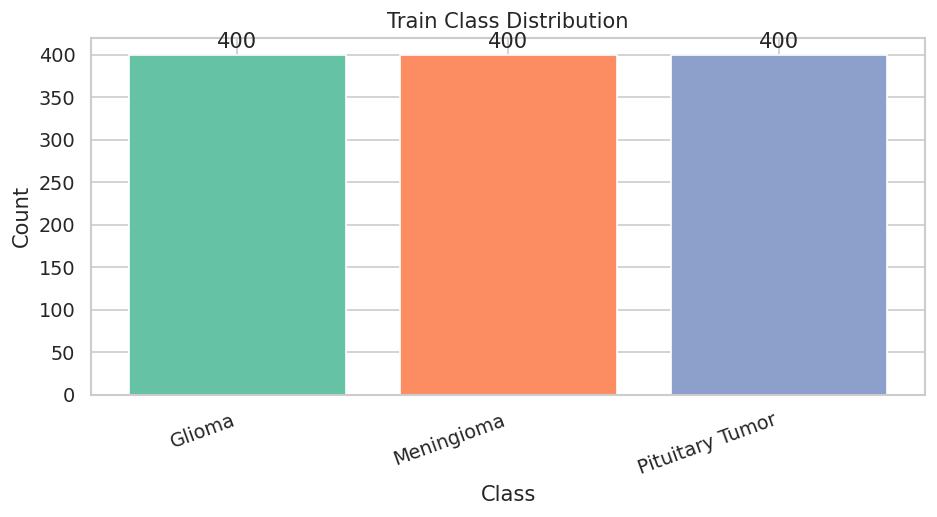
\includegraphics[width=\linewidth]{class_balance_train.png}
    \vspace{0.2em}

    {\scriptsize Class distribution (train split).}
  \end{columns}
\end{frame}

\note{
Balanced dataset with 400 training and 100 test samples per class.
This allows fair comparison across tumor types.
}

% Slide 4 — Methodology Overview
\begin{frame}{Methodology Overview}
  \begin{columns}[T,onlytextwidth]
    \column{0.55\textwidth}
    \centering
    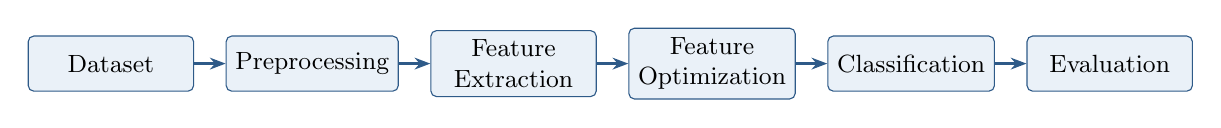
\begin{tikzpicture}[
      node distance=0.55cm and 0.4cm,
      box/.style={rectangle, rounded corners=2pt, draw=accent, fill=lightbg,
                  minimum height=0.7cm, minimum width=2.1cm, align=center, font=\small},
      arr/.style={-{Stealth[length=2mm]}, thick, accent}
    ]
      \node[box] (data) {Dataset};
      \node[box, right=of data] (prep) {Preprocessing};
      \node[box, right=of prep] (feat) {Feature\\Extraction};
      \node[box, right=of feat] (opt) {Feature\\Optimization};
      \node[box, right=of opt] (cls) {Classification};
      \node[box, right=of cls] (eval) {Evaluation};
      \draw[arr] (data) -- (prep);
      \draw[arr] (prep) -- (feat);
      \draw[arr] (feat) -- (opt);
      \draw[arr] (opt) -- (cls);
      \draw[arr] (cls) -- (eval);
    \end{tikzpicture}

    \column{0.43\textwidth}
    \begin{block}{Phase 1: Feature engineering}
      \small We search \NPhaseOneConfigs{} descriptor configurations and select the best parameters using
      separability metrics (FDR, MI, DBI) \emph{without} training classifiers.
    \end{block}

    \begin{block}{Phase 2: ML benchmark}
      \small Freeze the optimized descriptors, then tune and compare \NModels{} classifiers across
      \NFeatureSets{} feature sets. Report held-out test performance + statistical validation.
    \end{block}
  \end{columns}

  \vspace{0.3em}
  \centering
  
\includegraphics[width=0.92\linewidth,height=0.40\textheight,keepaspectratio]{p2_overall_dashboard.png}
  \vspace{0.1em}

  {\scriptsize Dashboard summarizing Phase 2 performance and training time.}
\end{frame}

\note{
Two-phase design: Phase 1 selects optimal descriptor parameters via separability metrics;
Phase 2 benchmarks eight classifiers across eight feature-set combinations.
}

% Slide 5 — Preprocessing
\begin{frame}{Preprocessing}
  \begin{columns}[T,onlytextwidth]
    \column{0.56\textwidth}
    \centering
    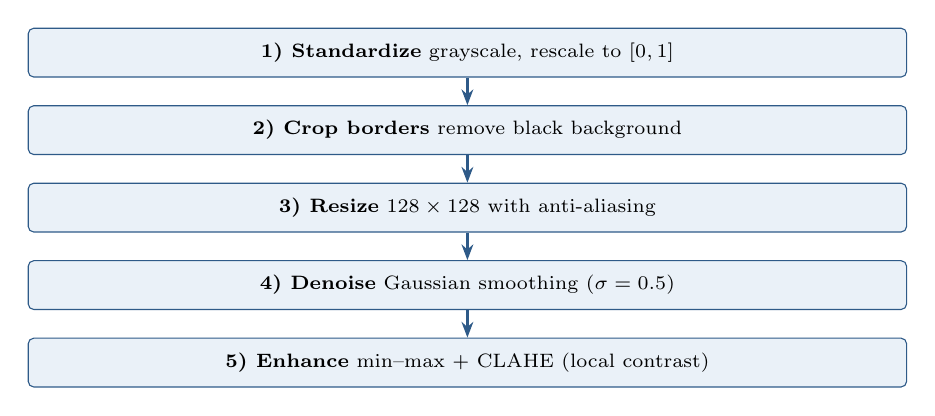
\begin{tikzpicture}[
      node distance=0.35cm,
      box/.style={rectangle, rounded corners=2pt, draw=accent, fill=lightbg,
                  minimum height=0.62cm, minimum width=0.92\linewidth,
                  align=left, font=\scriptsize, inner xsep=0.35em},
      arr/.style={-{Stealth[length=2mm]}, thick, accent}
    ]
      \node[box] (a) {\textbf{1) Standardize} \hfill grayscale, rescale to $[0,1]$};
      \node[box, below=of a] (b) {\textbf{2) Crop borders} \hfill remove black background};
      \node[box, below=of b] (c) {\textbf{3) Resize} \hfill \ImgSize{} with anti-aliasing};
      \node[box, below=of c] (d) {\textbf{4) Denoise} \hfill Gaussian smoothing ($\sigma=0.5$)};
      \node[box, below=of d] (e) {\textbf{5) Enhance} \hfill min--max + CLAHE (local contrast)};
      \draw[arr] (a) -- (b);
      \draw[arr] (b) -- (c);
      \draw[arr] (c) -- (d);
      \draw[arr] (d) -- (e);
    \end{tikzpicture}

    \vspace{0.4em}
    \scriptsize
    \begin{tabular}{@{}ll@{}}
      \toprule
      \textbf{Key setting} & \textbf{Value} \\
      \midrule
      Target size & \ImgSize{} \\
      Smoothing & $\sigma = 0.5$ \\
      Contrast & CLAHE (local) \\
      \bottomrule
    \end{tabular}

    \column{0.42\textwidth}
    \begin{block}{Why this matters}
      \small Preprocessing reduces acquisition variability and stabilizes the
      downstream descriptors (LBP texture, HOG gradients, DWT frequency).
    \end{block}

    \centering
    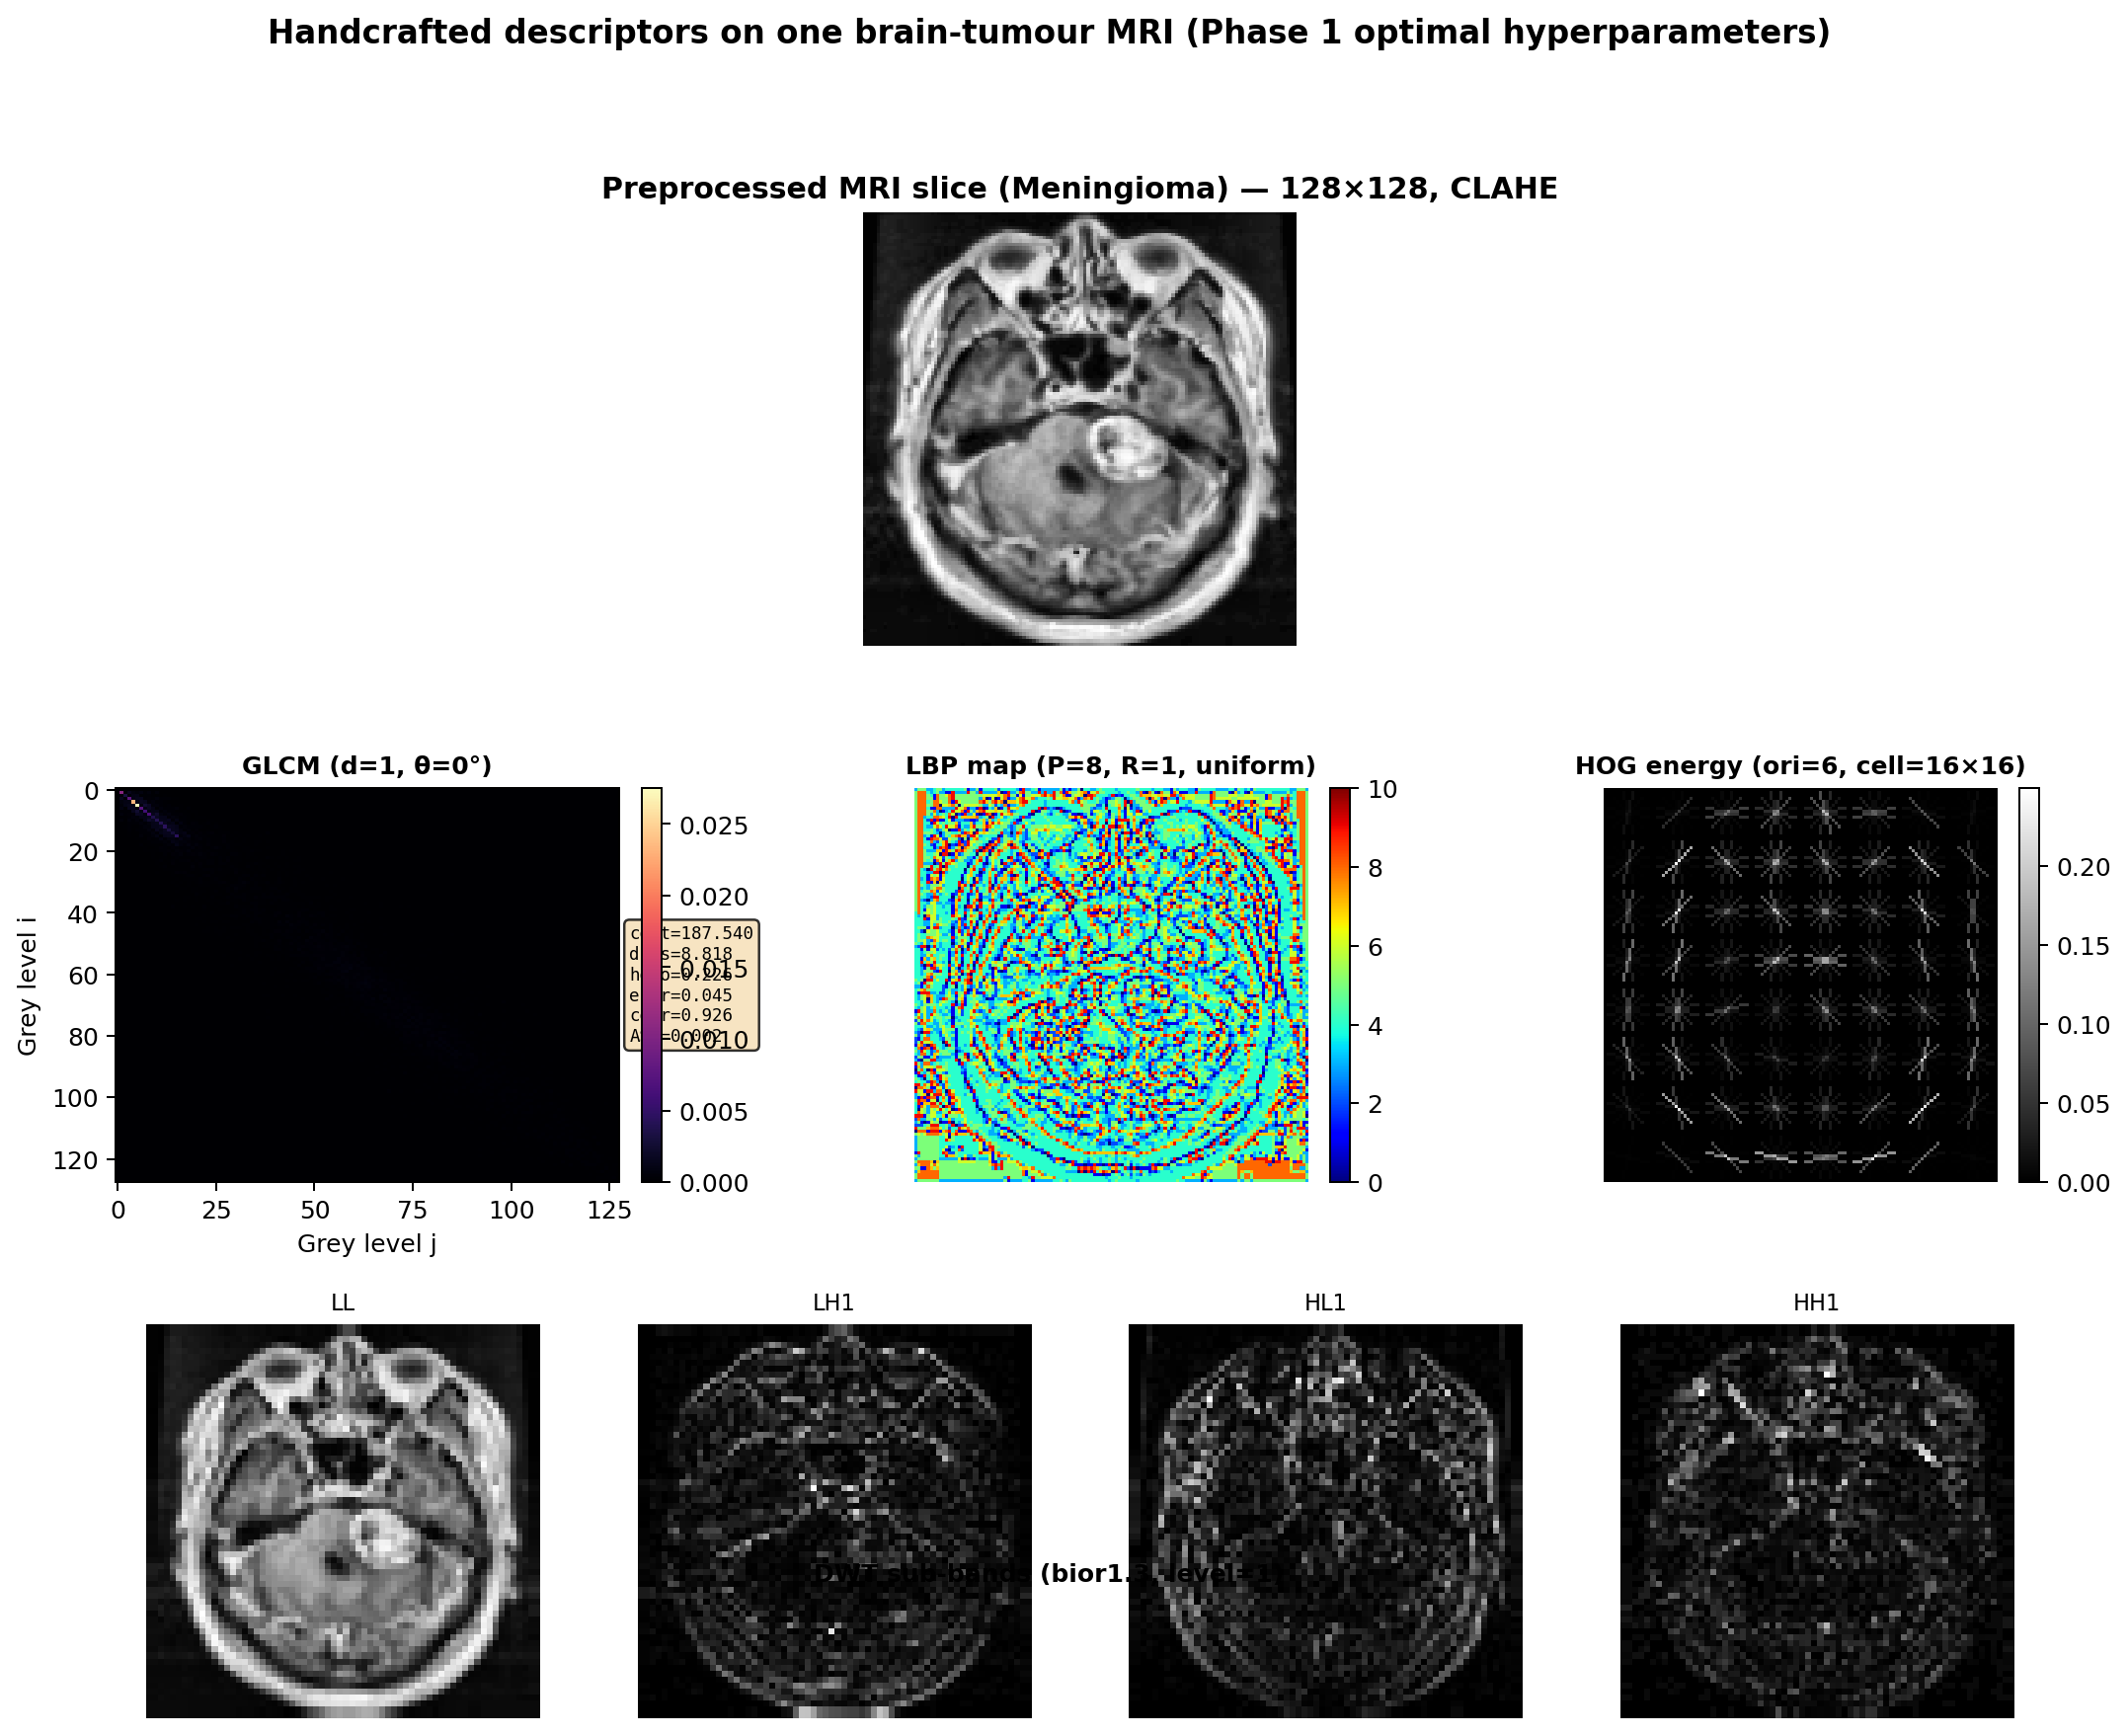
\includegraphics[width=\linewidth,height=0.40\textheight,keepaspectratio,trim=130 520 130 70,clip]{descriptor_demo.png}

    {\scriptsize Example preprocessed slice (CLAHE, \ImgSize{}).}
  \end{columns}
\end{frame}

\note{
Preprocessing is lightweight and fully reproducible. CLAHE improves local contrast
without changing global intensity statistics dramatically.
}

% Slide 6 — Feature Extraction Methods
\begin{frame}[shrink=6]{Feature Extraction Methods}
  \begin{columns}[T,onlytextwidth]
    \column{0.49\textwidth}
    \begin{block}{A) Statistical features (intensity)}
      \centering
      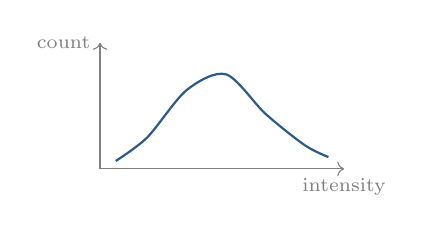
\begin{tikzpicture}[x=1cm,y=1cm]
        \draw[->,gray] (0,0) -- (3.1,0) node[below] {\scriptsize intensity};
        \draw[->,gray] (0,0) -- (0,1.6) node[left] {\scriptsize count};
        \draw[accent,thick] plot[smooth] coordinates {(0.2,0.1) (0.6,0.4) (1.1,1.0) (1.6,1.2) (2.1,0.7) (2.6,0.3) (2.9,0.15)};
      \end{tikzpicture}
      \vspace{-0.2em}

      \scriptsize Compact summary of intensity distribution: mean, std, entropy,
      skew/kurtosis, and percentiles (p10--p90).
    \end{block}

    \begin{block}{B) LBP (local texture)}
      \centering
      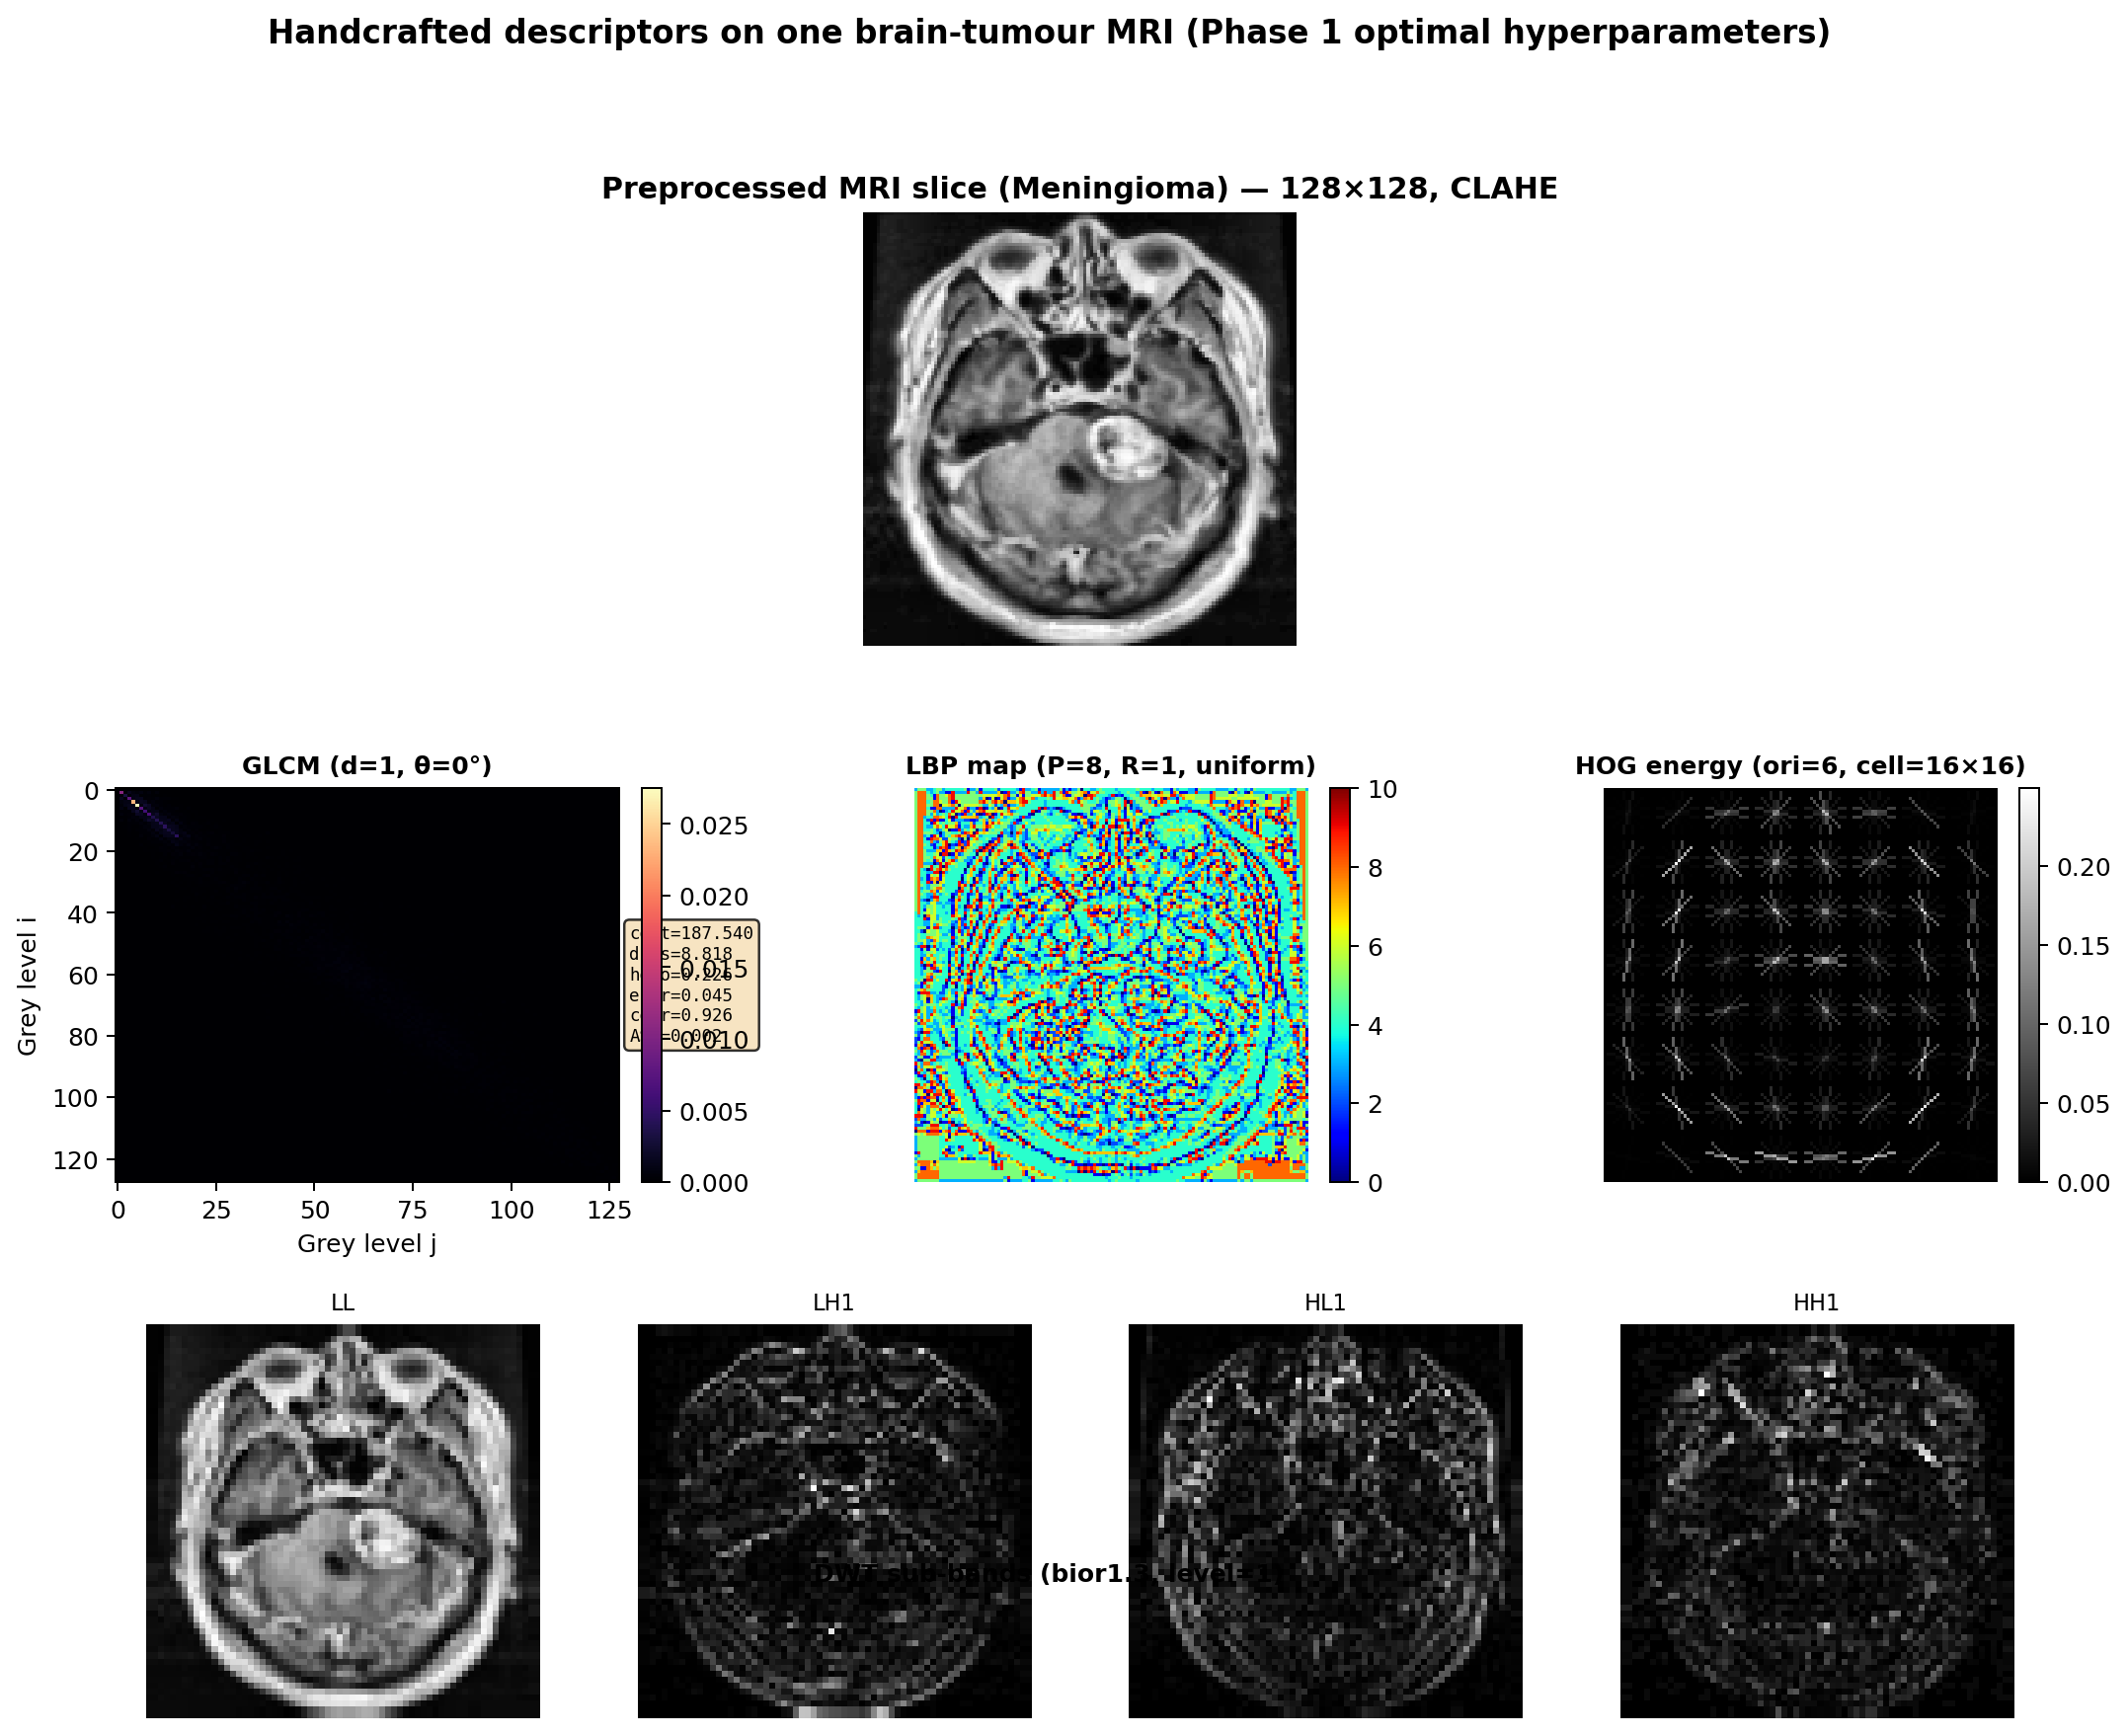
\includegraphics[width=\linewidth,height=0.19\textheight,keepaspectratio,trim=345 250 340 360,clip]{descriptor_demo.png}
      \vspace{-0.2em}

      \scriptsize Encodes local micro-patterns; robust texture fingerprint for tumor tissue.
    \end{block}

    \column{0.49\textwidth}
    \begin{block}{C) DWT (frequency sub-bands)}
      \centering
      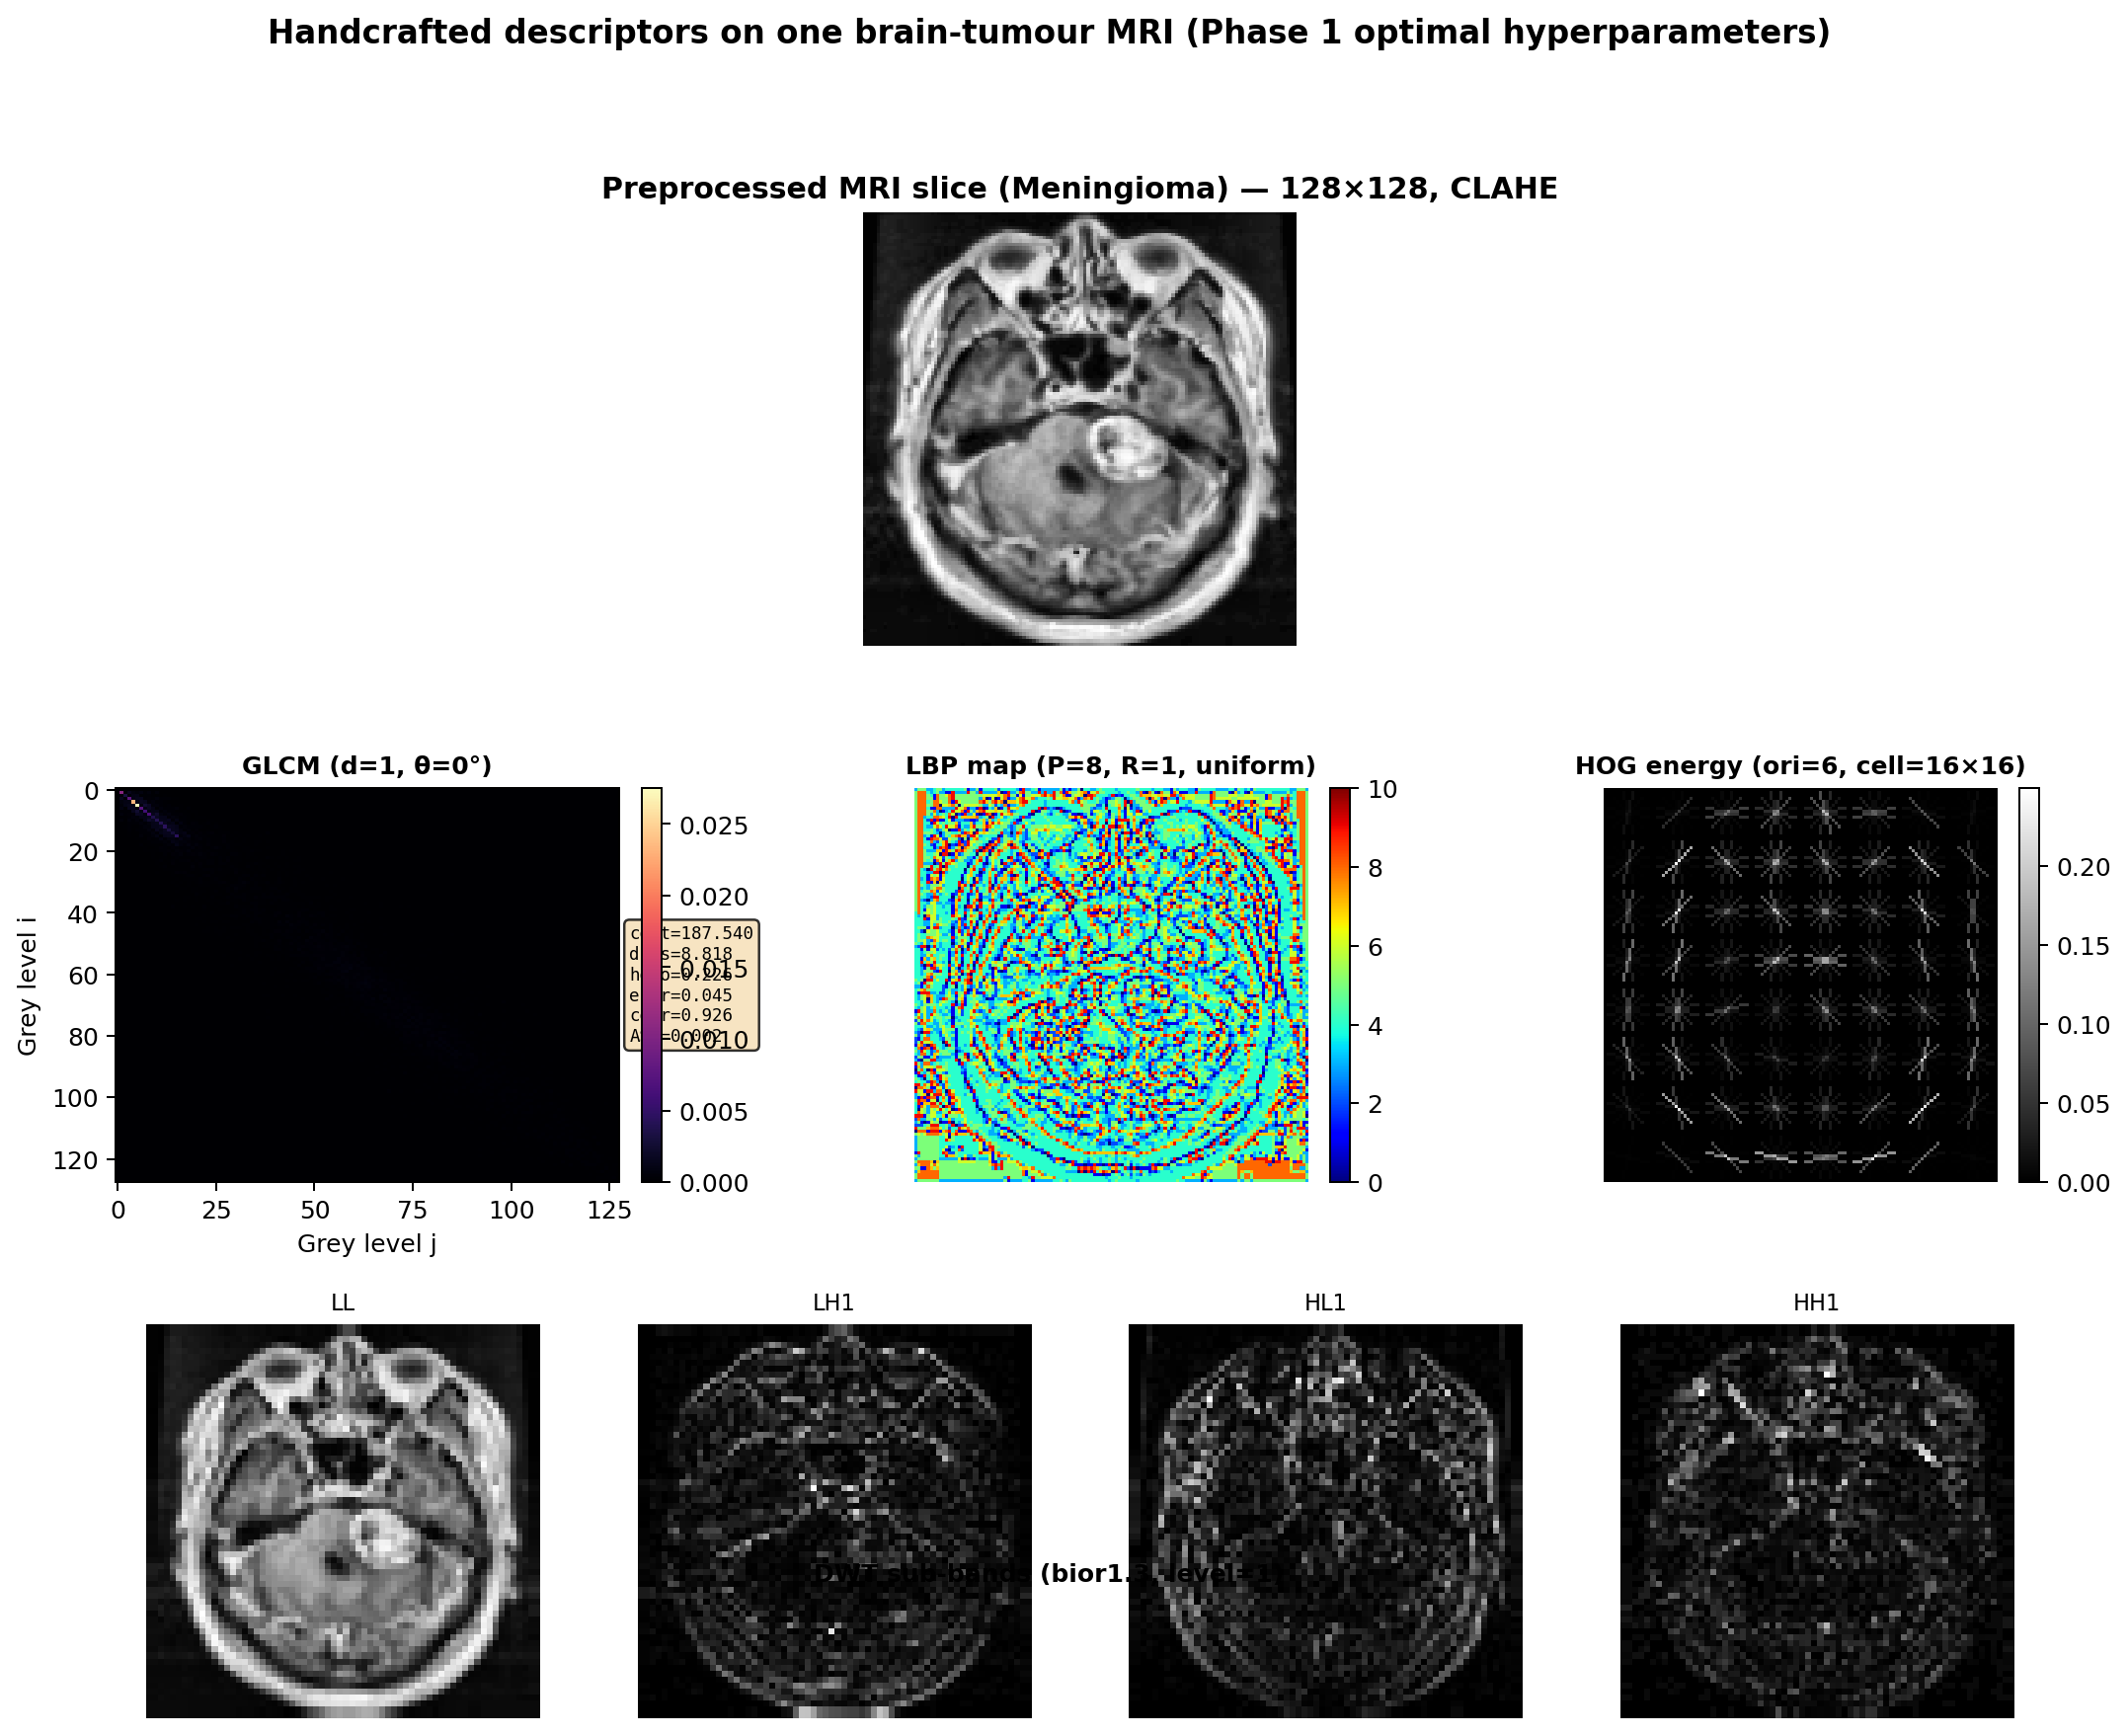
\includegraphics[width=\linewidth,height=0.19\textheight,keepaspectratio,trim=60 0 60 585,clip]{descriptor_demo.png}
      \vspace{-0.2em}

      \scriptsize Multi-scale decomposition (LL/LH/HL/HH) captures coarse vs. fine structures.
    \end{block}

    \begin{block}{D) HOG (edges \& shape)}
      \centering
      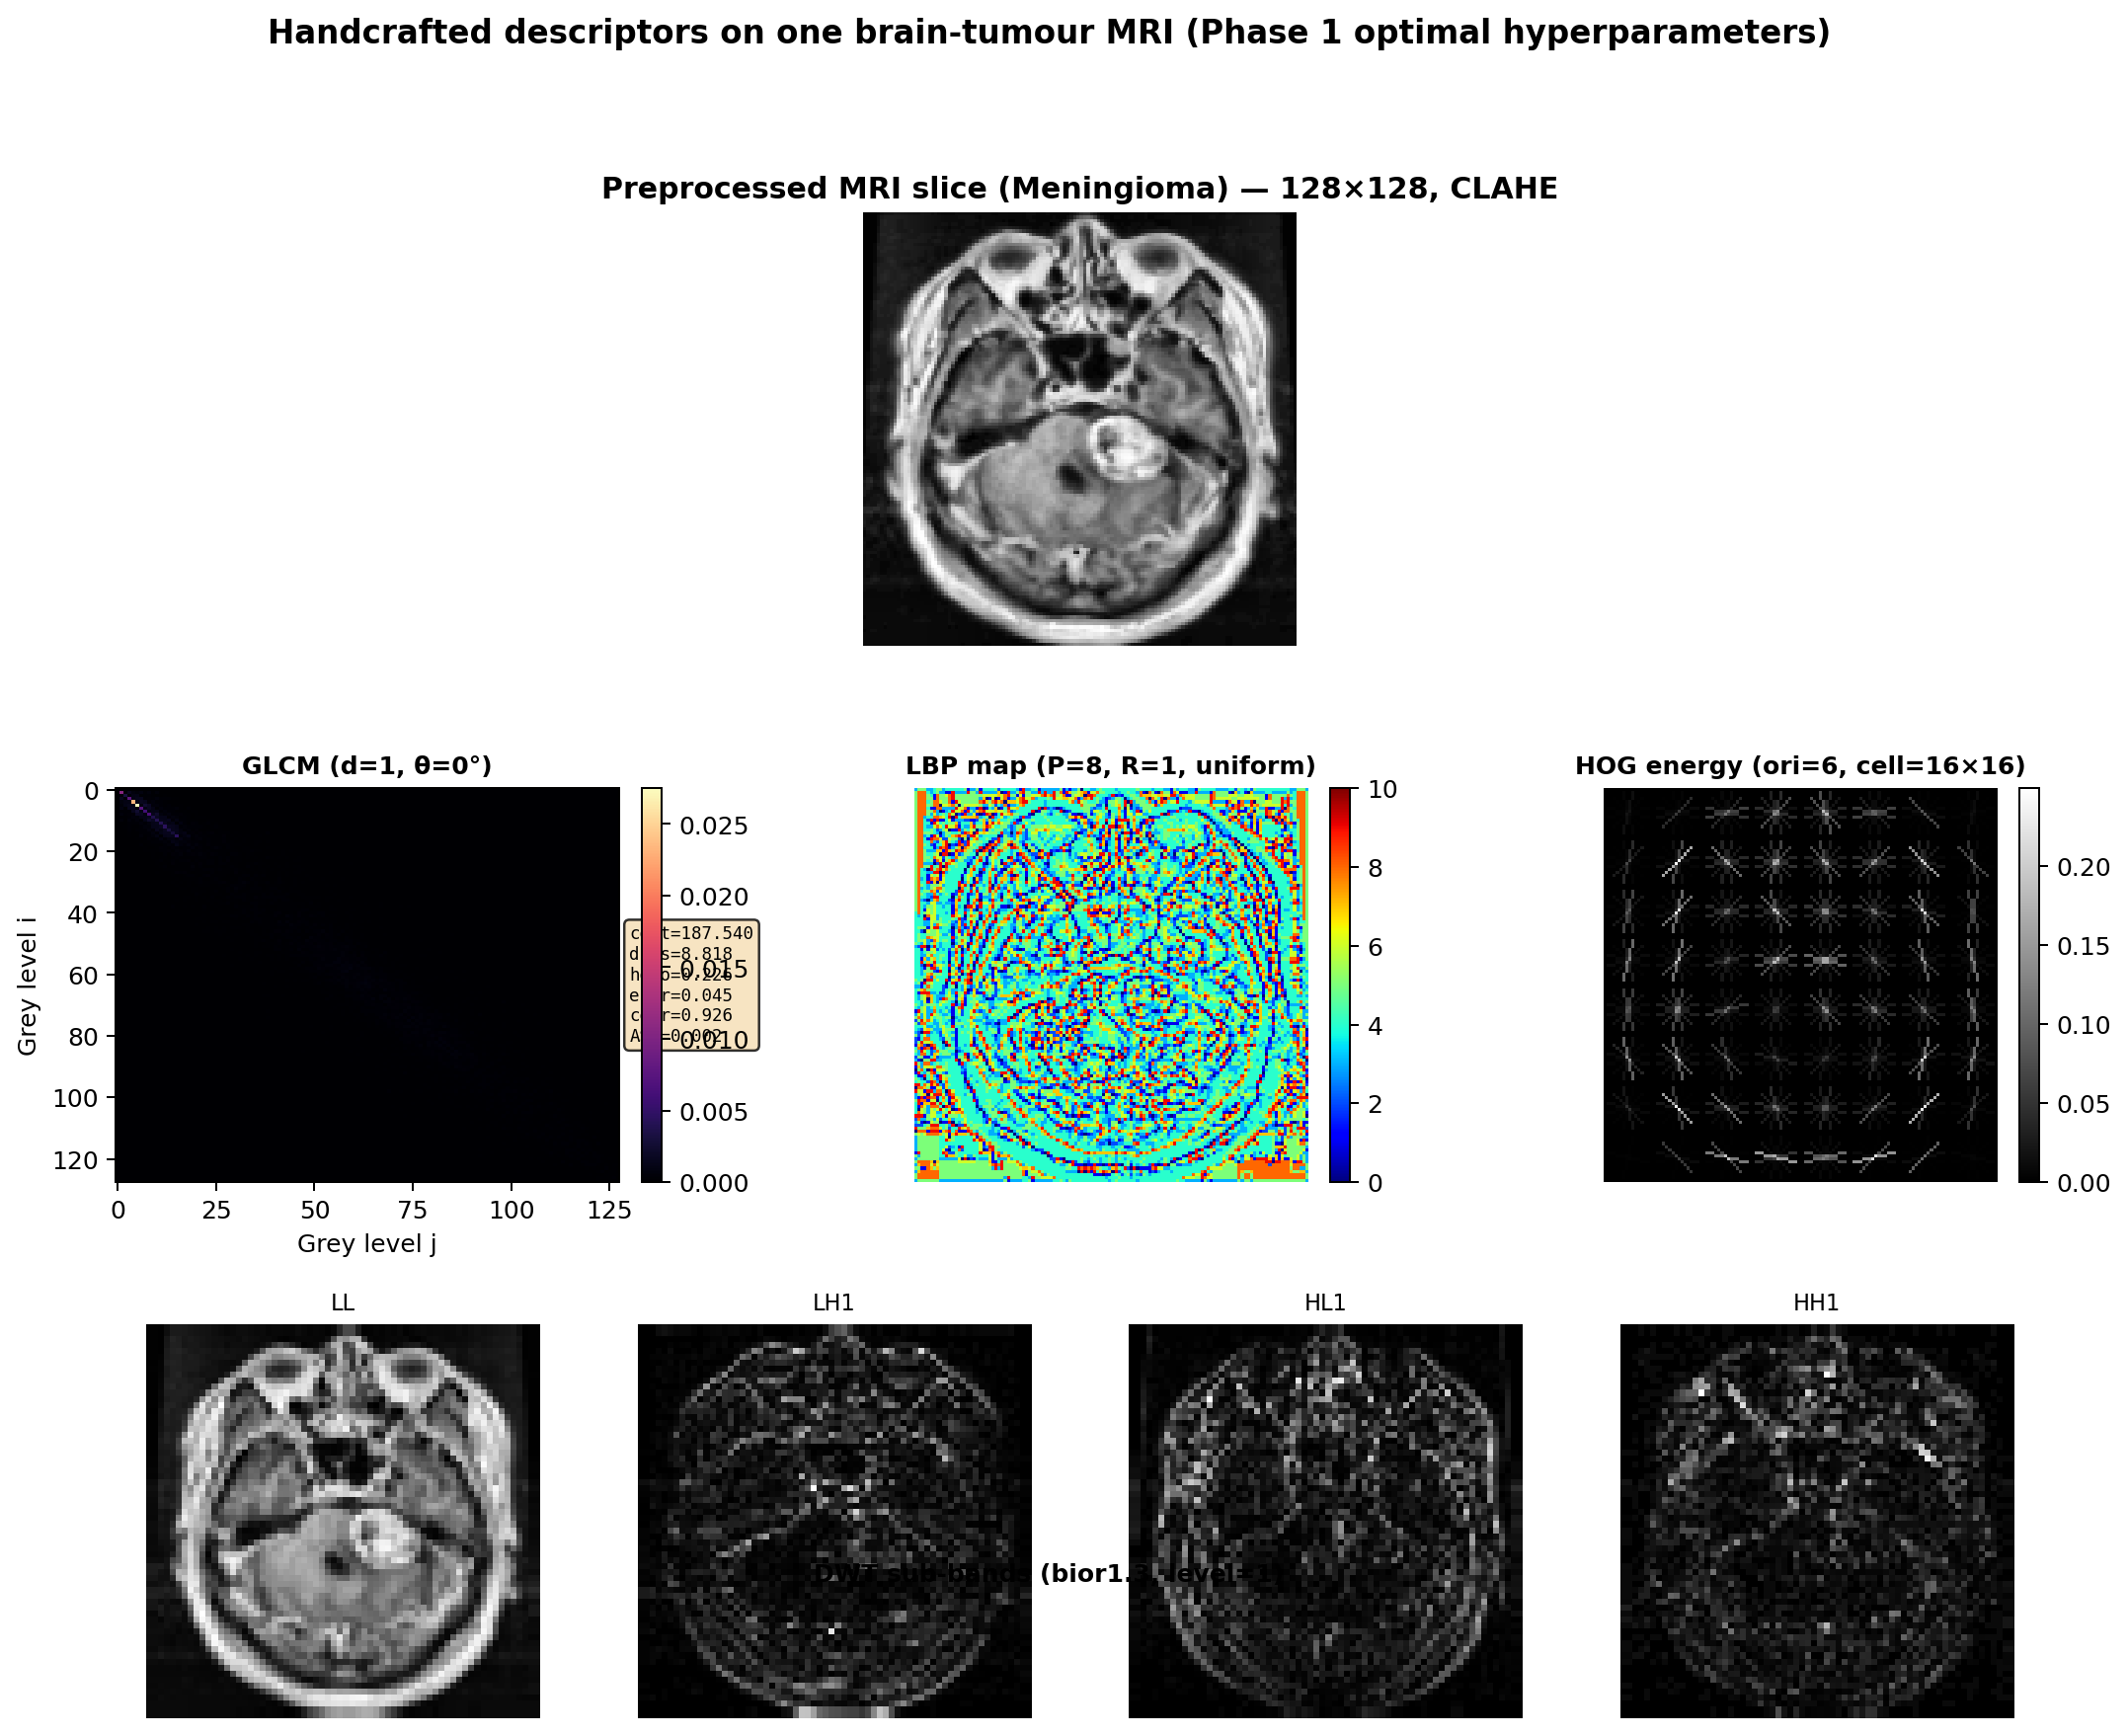
\includegraphics[width=\linewidth,height=0.19\textheight,keepaspectratio,trim=685 250 60 360,clip]{descriptor_demo.png}
      \vspace{-0.2em}

      \scriptsize Aggregates gradient orientations; strong for boundary/shape cues.
    \end{block}
  \end{columns}

  \vspace{-0.2em}
  \centering
  {\scriptsize Four complementary views of the same slice: intensity, texture, frequency, and gradients.}
\end{frame}

\note{
Each family captures a different aspect of tumor appearance.
They are later fused after individual optimization.
}

% Slide 7 — Optimization Strategy
\begin{frame}{Optimization Strategy}
  \begin{columns}[T,onlytextwidth]
    \column{0.55\textwidth}
    \begin{block}{Key idea}
      \small We avoid training classifiers for all \NPhaseOneConfigs{} configurations.\vspace{0.3em}

      Instead, we select descriptor parameters using a \textbf{separability score} computed directly
      from the feature vectors:
      \[
        \text{Score}=\frac{1}{3}\Big(\widehat{\text{FDR}}+\widehat{\text{MI}}+\big(1-\widehat{\text{DBI}}\big)\Big)
      \]
      where hats denote min--max normalization across the search grid.
    \end{block}

    \begin{block}{Why it works}
      \small High separability indicates class-specific structure before choosing a classifier,
      reducing the Phase 2 search space while improving feature quality.
    \end{block}

    \column{0.43\textwidth}
    \centering
    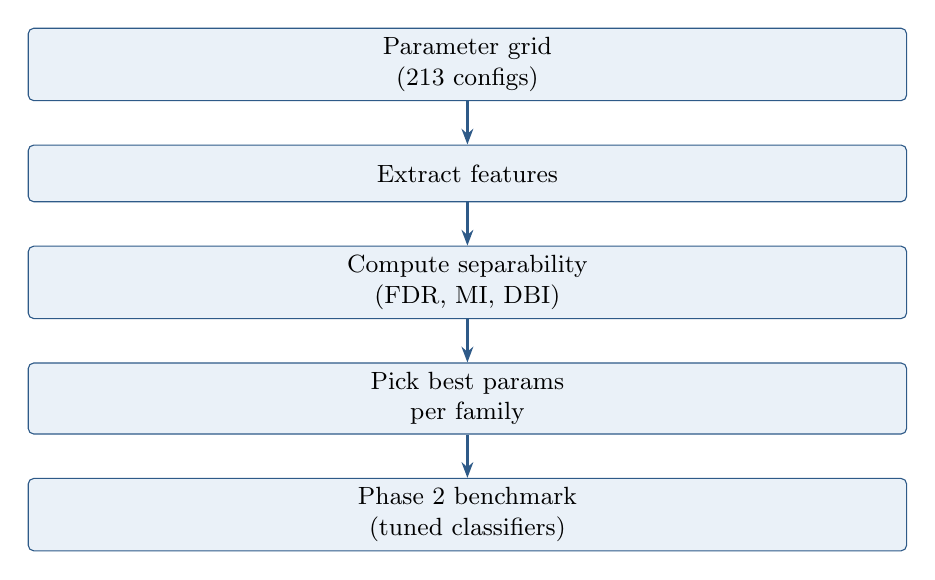
\begin{tikzpicture}[
      node distance=0.55cm,
      box/.style={rectangle, rounded corners=2pt, draw=accent, fill=lightbg,
                  minimum height=0.72cm, minimum width=0.92\linewidth, align=center, font=\small},
      arr/.style={-{Stealth[length=2mm]}, thick, accent}
    ]
      \node[box] (grid) {Parameter grid\\(\NPhaseOneConfigs{} configs)};
      \node[box, below=of grid] (feat) {Extract features};
      \node[box, below=of feat] (score) {Compute separability\\(FDR, MI, DBI)};
      \node[box, below=of score] (pick) {Pick best params\\per family};
      \node[box, below=of pick] (bench) {Phase 2 benchmark\\(tuned classifiers)};
      \draw[arr] (grid) -- (feat);
      \draw[arr] (feat) -- (score);
      \draw[arr] (score) -- (pick);
      \draw[arr] (pick) -- (bench);
    \end{tikzpicture}

    \vspace{0.3em}
    \scriptsize
    \begin{tabular}{@{}ll@{}}
      \toprule
      \textbf{Metric} & \textbf{Meaning} \\
      \midrule
      FDR & class separation in feature space \\
      MI & information about the label \\
      DBI & cluster compactness / overlap \\
      \bottomrule
    \end{tabular}
  \end{columns}
\end{frame}

\note{
Composite separability score = mean of normalized FDR, MI, and inverted DBI.
Best config per family is frozen for all Phase 2 experiments.
}

% Slide 8 — LBP Optimization Results
\begin{frame}[shrink=4]{LBP Optimization Results}
  \begin{columns}[T,onlytextwidth]
    \column{0.62\textwidth}
    \centering
    
\includegraphics[width=\linewidth,height=0.62\textheight,keepaspectratio]{lbp_param_search.png}

    \column{0.36\textwidth}
    \begin{block}{Selected configuration}
      \small
      \begin{tabular}{@{}ll@{}}
        \toprule
        Neighbors ($P$) & 12 \\
        Radius ($R$) & 1 \\
        Encoding & \texttt{uniform} \\
        \midrule
        Separability & \lbpScore \\
        \bottomrule
      \end{tabular}
    \end{block}

    \begin{block}{Takeaway}
      \small A small radius captures fine-grained micro-texture around tumor boundaries.
      Uniform encoding generalizes better by compressing patterns into a compact histogram.
    \end{block}
  \end{columns}
\end{frame}

\note{
Grid searched P in {4,8,12,16}, R in {1,2,3}, and three encoding methods.
Uniform LBP at P=12, R=1 is the clear winner.
}

% Slide 9 — LBP Comparison
\begin{frame}[shrink=4]{LBP Method Comparison}
  \begin{columns}[T,onlytextwidth]
    \column{0.62\textwidth}
    \centering
    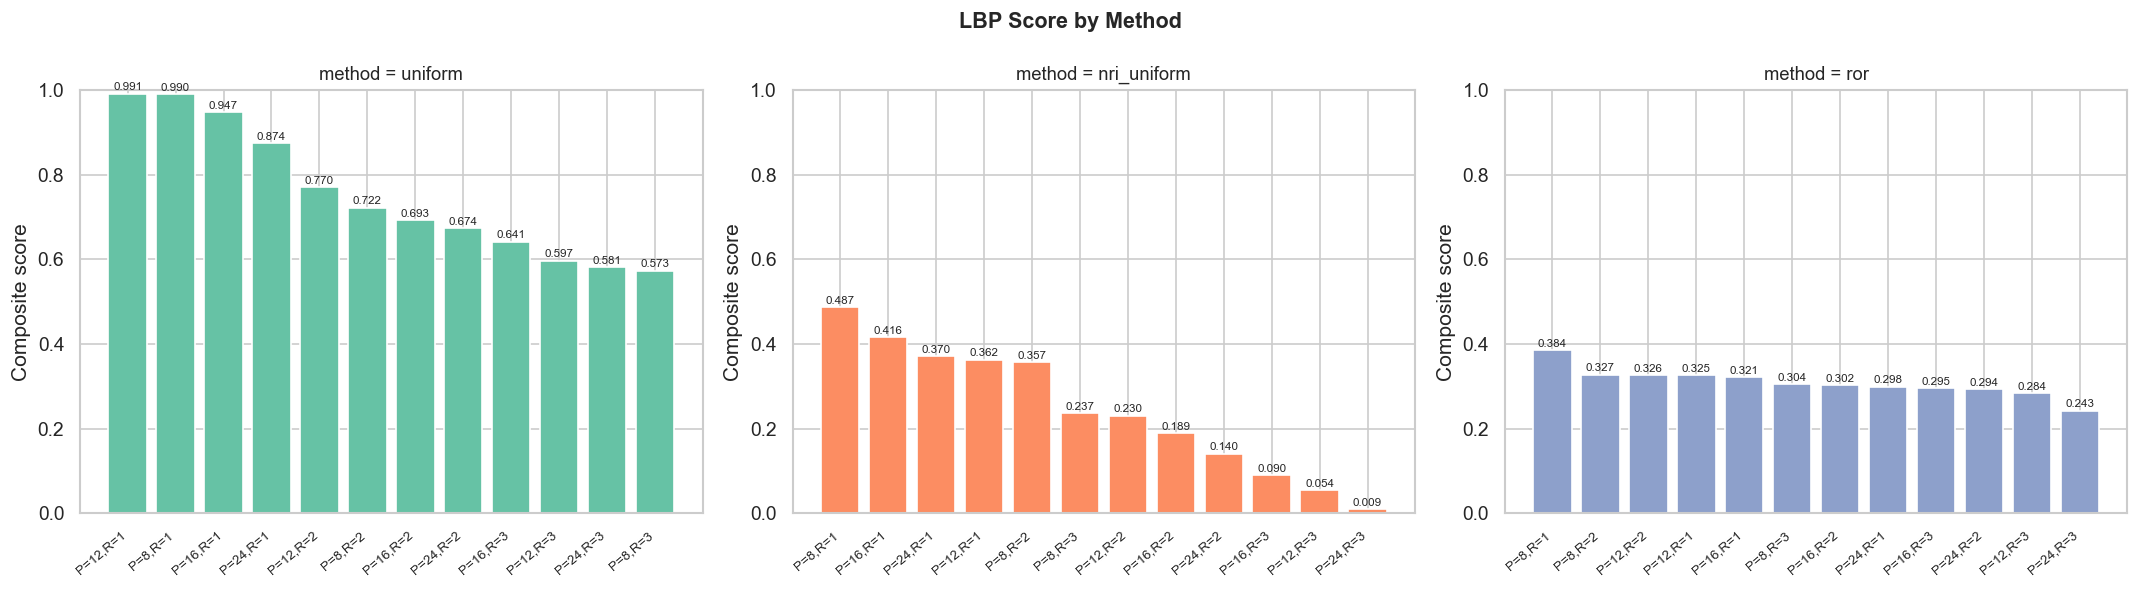
\includegraphics[width=\linewidth,height=0.62\textheight,keepaspectratio]{lbp_by_method.png}

    \column{0.36\textwidth}
    \begin{block}{Methods compared}
      \small
      \begin{tabular}{@{}ll@{}}
        \toprule
        \textbf{Encoding} & \textbf{Property} \\
        \midrule
        \texttt{uniform} & compact + robust \\
        \texttt{nri\_uniform} & less invariant \\
        \texttt{ror} & rotation-invariant \\
        \bottomrule
      \end{tabular}
    \end{block}

    \begin{block}{Decision}
      \small \texttt{uniform} wins consistently across $(P,R)$ settings.\vspace{0.2em}

      \keyresult{Selected for Phase 2 branch B.}
    \end{block}

    \begin{block}{Takeaway}
      \small Compact, rotation-tolerant patterns generalize best under inter-patient MRI variability.
    \end{block}
  \end{columns}
\end{frame}

\note{
Uniform encoding reduces histogram dimensionality while preserving discriminative texture.
This is the method retained for Phase 2 branch B.
}

% Slide 10 — DWT Optimization
\begin{frame}[shrink=4]{DWT Optimization Results}
  \begin{columns}[T,onlytextwidth]
    \column{0.62\textwidth}
    \centering
    
\includegraphics[width=\linewidth,height=0.62\textheight,keepaspectratio]{dwt_param_search.png}

    \column{0.36\textwidth}
    \begin{block}{Search space}
      \small
      \begin{tabular}{@{}ll@{}}
        \toprule
        Wavelets & 7 families \\
        Levels & 1--3 \\
        Total & 21 configs \\
        \bottomrule
      \end{tabular}
    \end{block}

    \begin{block}{Selected configuration}
      \small
      \begin{tabular}{@{}ll@{}}
        \toprule
        Wavelet & \texttt{db2} \\
        Level & 1 \\
        \midrule
        Separability & \dwtScore \\
        \bottomrule
      \end{tabular}
    \end{block}

    \begin{block}{Takeaway}
      \small \texttt{db2} at level 1 captures discriminative mid-frequency structure
      without over-fragmenting the image signal.
    \end{block}
  \end{columns}
\end{frame}

\note{
Tested haar, db1, db2, db4, sym2, coif1, bior1.3 at levels 1--3.
db2 level 1 selected for Phase 2 branch C.
}

% Slide 11 — DWT Wavelet Comparison
\begin{frame}[shrink=4]{DWT Wavelet Comparison}
  \begin{columns}[T,onlytextwidth]
    \column{0.62\textwidth}
    \centering
    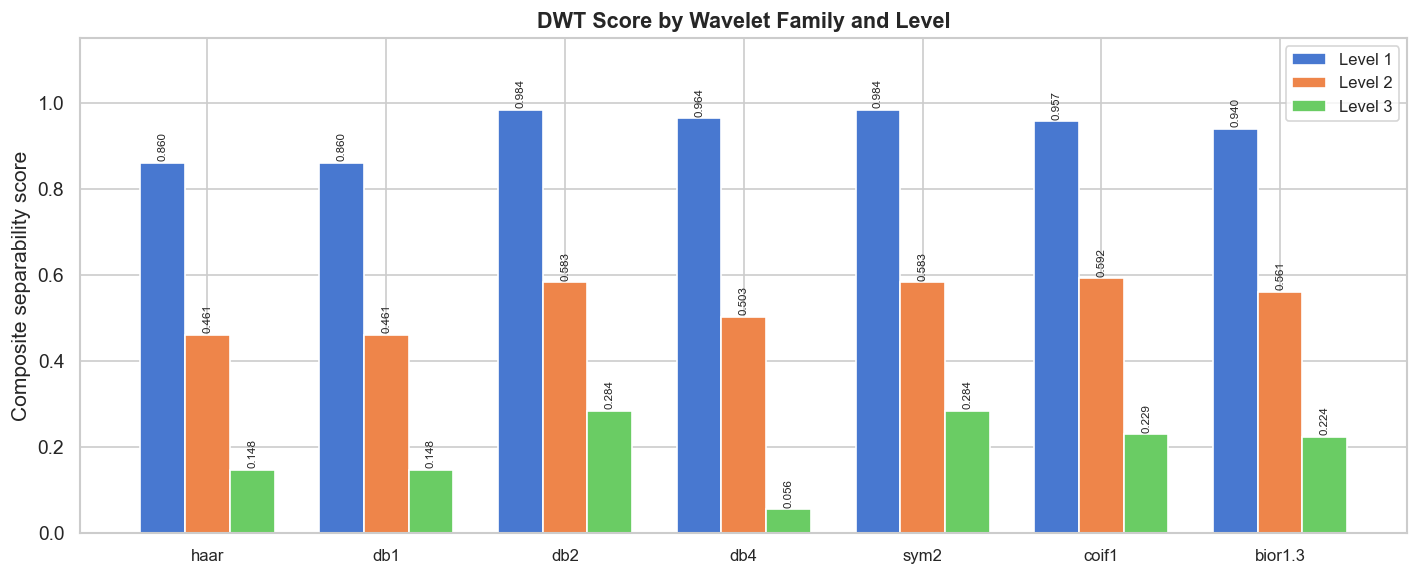
\includegraphics[width=\linewidth,height=0.62\textheight,keepaspectratio]{dwt_wavelet_comparison.png}

    \column{0.36\textwidth}
    \begin{block}{How to read this}
      \small We compare wavelet families under the same evaluation protocol.\vspace{0.3em}

      \textbf{Goal:} maximize separability while keeping representation compact.
    \end{block}

    \begin{block}{Winner}
      \small \keyresult{\texttt{db2}} provides the strongest overall separability.\vspace{0.2em}

      Interpretation: medium-frequency bands capture tumor tissue heterogeneity
      better than very coarse (haar) or overly complex families.
    \end{block}
  \end{columns}
\end{frame}

\note{
Wavelet choice affects which frequency bands contribute to classification.
db2 was selected as the optimal compromise.
}

% Slide 12 — Phase 1 Summary
\begin{frame}[shrink=5]{Phase 1 Summary}
  \begin{columns}[T,onlytextwidth]
    \column{0.48\textwidth}
    \begin{block}{Selected parameters (frozen for Phase 2)}
      \begin{table}
\centering
\footnotesize
\begin{tabular}{@{}l l c@{}}
\toprule
\textbf{Feature} & \textbf{Best parameters} & \textbf{Separability} \\
\midrule
Statistics & \statsParams{} & --- \\
LBP        & \lbpParams{}     & \lbpScore \\
DWT        & \dwtParams{}     & \dwtScore \\
HOG        & \hogParams{}     & \hogScore \\
\bottomrule
\end{tabular}
\end{table}

    \end{block}

    \begin{block}{Key observation}
      \small Texture (LBP) and gradients (HOG) achieve the highest separability.\vspace{0.2em}

      This motivates using them as strong baselines and testing whether fusion adds value.
    \end{block}
    \column{0.50\textwidth}
    \centering
    
\includegraphics[width=\linewidth]{phase1_summary.png}
  \end{columns}
\end{frame}

\note{
Phase 1 complete. All four feature families are ready for classifier benchmarking.
Key takeaway: texture and gradient descriptors dominate separability scores.
}

% Slide 13 — Feature Sets Evaluated
\begin{frame}[shrink=2]{Feature Sets Evaluated}
  \begin{columns}[T,onlytextwidth]
    \column{0.54\textwidth}
    \begin{block}{Building blocks (single families)}
      \small
      \begin{tabular}{@{}clp{0.55\linewidth}@{}}
        \toprule
        \textbf{ID} & \textbf{Name} & \textbf{Signal captured} \\
        \midrule
        A & Statistics & intensity distribution (11 features) \\
        B & LBP (opt) & local texture micro-patterns \\
        C & DWT (opt) & multi-scale frequency sub-bands \\
        D & HOG & edge/shape gradients \\
        \bottomrule
      \end{tabular}
    \end{block}

    \begin{block}{Fusion sets (incremental)}
      \small
      \begin{tabular}{@{}lp{0.70\linewidth}@{}}
        \toprule
        \textbf{Set} & \textbf{Purpose} \\
        \midrule
        A+B & add texture to intensity \\
        B+C(opt) & combine texture + frequency \\
        A+B+C(opt) & check synergy without HOG \\
        \textbf{Full(opt)} & all complementary cues \\
        \bottomrule
      \end{tabular}
    \end{block}

    \column{0.44\textwidth}
    \centering
    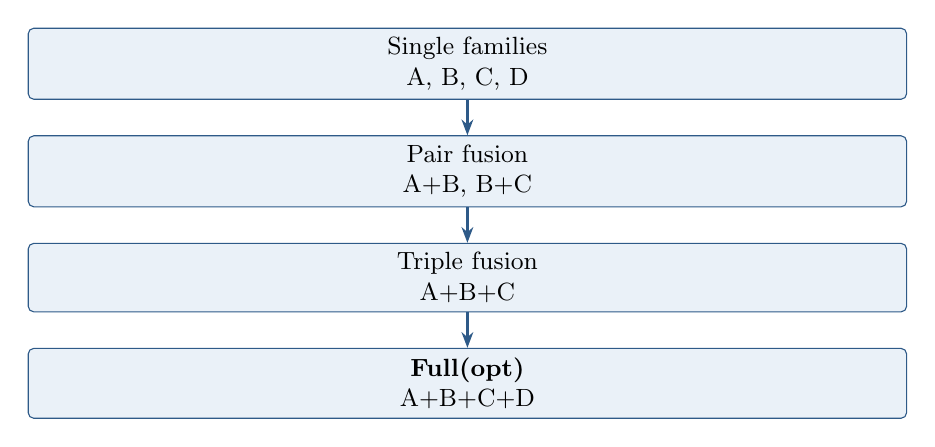
\begin{tikzpicture}[
      node distance=0.45cm,
      box/.style={rectangle, rounded corners=2pt, draw=accent, fill=lightbg,
                  minimum height=0.7cm, minimum width=0.92\linewidth, align=center, font=\small},
      arr/.style={-{Stealth[length=2mm]}, thick, accent}
    ]
      \node[box] (single) {Single families\\A, B, C, D};
      \node[box, below=of single] (pair) {Pair fusion\\A+B, B+C};
      \node[box, below=of pair] (triple) {Triple fusion\\A+B+C};
      \node[box, below=of triple] (full) {\textbf{Full(opt)}\\A+B+C+D};
      \draw[arr] (single) -- (pair);
      \draw[arr] (pair) -- (triple);
      \draw[arr] (triple) -- (full);
    \end{tikzpicture}

    \begin{block}{Rationale}
      \small Progressive fusion reveals which descriptors add complementary value beyond HOG.
    \end{block}
  \end{columns}
\end{frame}

\note{
Eight feature sets total. Full(opt) concatenates all optimized branches after
correlation pruning and scaling (526 cleaned features).
}

% Slide 14 — Classifiers Compared
\begin{frame}[shrink=3]{Classifiers Compared}
  \begin{columns}[T,onlytextwidth]
    \column{0.56\textwidth}
    \begin{block}{Model families (intuition)}
      \small
      \begin{tabular}{@{}p{0.26\linewidth}p{0.70\linewidth}@{}}
        \toprule
        \textbf{Family} & \textbf{Models in benchmark} \\
        \midrule
        Margin / kernel & SVM (captures non-linear boundaries) \\
        Instance-based & KNN (local neighborhoods) \\
        Tree ensembles & Random Forest, ExtraTrees (bagging) \\
        Boosted trees & XGBoost, LightGBM (strong tabular baselines) \\
        Linear baseline & Logistic Regression \\
        Shallow NN & MLP \\
        \bottomrule
      \end{tabular}
    \end{block}

    \begin{block}{Why compare many models?}
      \small Handcrafted features can favor different inductive biases:
      HOG often benefits from margin methods, while compact stats can suit trees/linear models.
    \end{block}

    \column{0.42\textwidth}
    \centering
    
\begin{tikzpicture}[
      node distance=0.5cm,
      box/.style={rectangle, rounded corners=2pt, draw=accent, fill=lightbg,
                  minimum height=0.7cm, minimum width=0.92\linewidth, align=center, font=\small},
      arr/.style={-{Stealth[length=2mm]}, thick, accent}
    ]
      \node[box] (fs) {Feature set (8)};
      \node[box, below=of fs] (grid) {GridSearchCV (5-fold)};
      \node[box, below=of grid] (test) {Held-out test};
      \draw[arr] (fs) -- (grid);
      \draw[arr] (grid) -- (test);
    \end{tikzpicture}

    \vspace{0.4em}
    {\small \NModels{} models $\times$ \NFeatureSets{} sets = \keyresult{\NRuns{}} tuned configurations.}
  \end{columns}
\end{frame}

\note{
No algorithm math here --- just roles. Each classifier has different inductive bias
for high-dimensional handcrafted features.
}

% Slide 15 — Evaluation Metrics
\begin{frame}[shrink=2]{Evaluation Metrics}
  \begin{columns}[T,onlytextwidth]
    \column{0.56\textwidth}
    \begin{block}{What we measure (macro-averaged)}
      \small
      \begin{tabular}{@{}p{0.22\linewidth}p{0.72\linewidth}@{}}
        \toprule
        \textbf{Metric} & \textbf{Why it matters} \\
        \midrule
        Accuracy & overall correctness \\
        Precision & avoid false positives (per class) \\
        Recall & avoid missed tumors (per class) \\
        F1-macro & balances precision/recall equally across classes \\
        $\kappa$ & agreement beyond chance (robustness) \\
        \bottomrule
      \end{tabular}
    \end{block}

    \begin{block}{Ranking criterion}
      \small We primarily rank configurations by \keyresult{macro-F1} to ensure fair
      performance across the three tumor classes.
    \end{block}

    \column{0.42\textwidth}
    \centering
    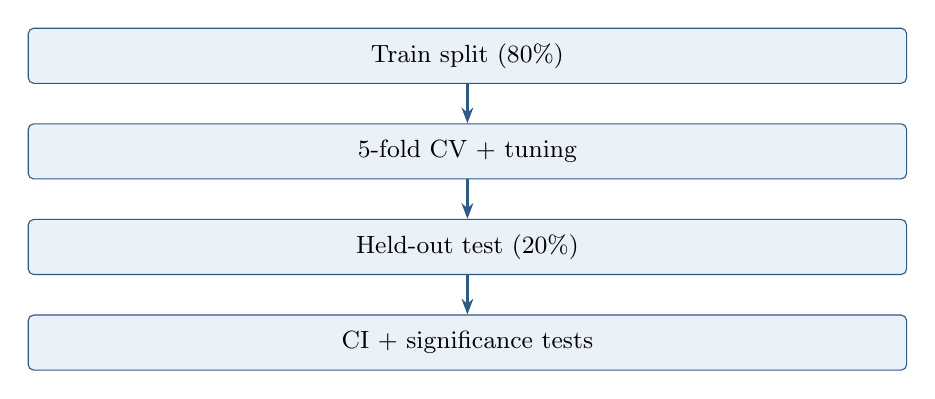
\begin{tikzpicture}[
      node distance=0.5cm,
      box/.style={rectangle, rounded corners=2pt, draw=accent, fill=lightbg,
                  minimum height=0.7cm, minimum width=0.92\linewidth, align=center, font=\small},
      arr/.style={-{Stealth[length=2mm]}, thick, accent}
    ]
      \node[box] (train) {Train split (80\%)}; 
      \node[box, below=of train] (cv) {5-fold CV + tuning};
      \node[box, below=of cv] (test) {Held-out test (20\%)};
      \node[box, below=of test] (stats) {CI + significance tests};
      \draw[arr] (train) -- (cv);
      \draw[arr] (cv) -- (test);
      \draw[arr] (test) -- (stats);
    \end{tikzpicture}

    \vspace{0.3em}
    {\scriptsize Bootstrap CI, McNemar (paired test errors), Friedman (multi-model comparison).}
  \end{columns}
\end{frame}

\note{
Macro averaging treats all tumor classes equally --- important for clinical fairness.
F1-macro is the primary ranking metric.
}

% Slide 16 — Individual Feature Results
\begin{frame}[shrink=5]{Individual Feature Results}
  \centering
  \begin{columns}[T,onlytextwidth]
    \column{0.48\textwidth}
    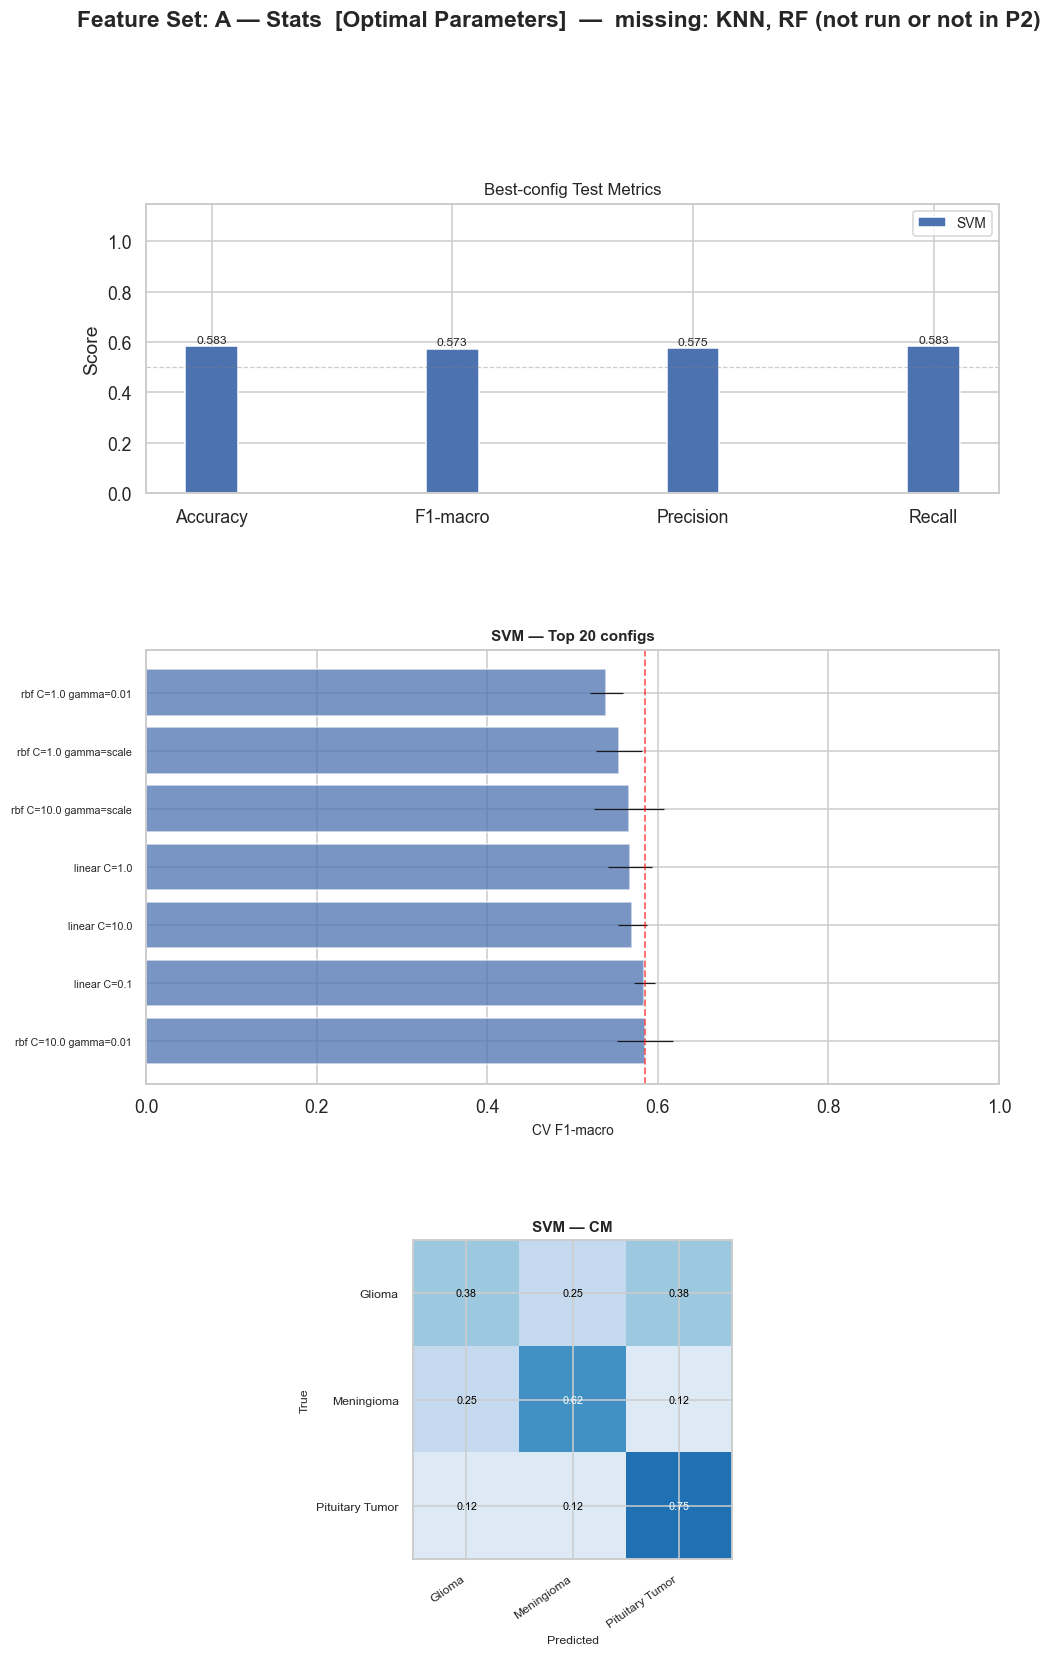
\includegraphics[width=\linewidth,height=0.30\textheight,keepaspectratio]{p2_A_—_Stats.png}\\[0.1em]
    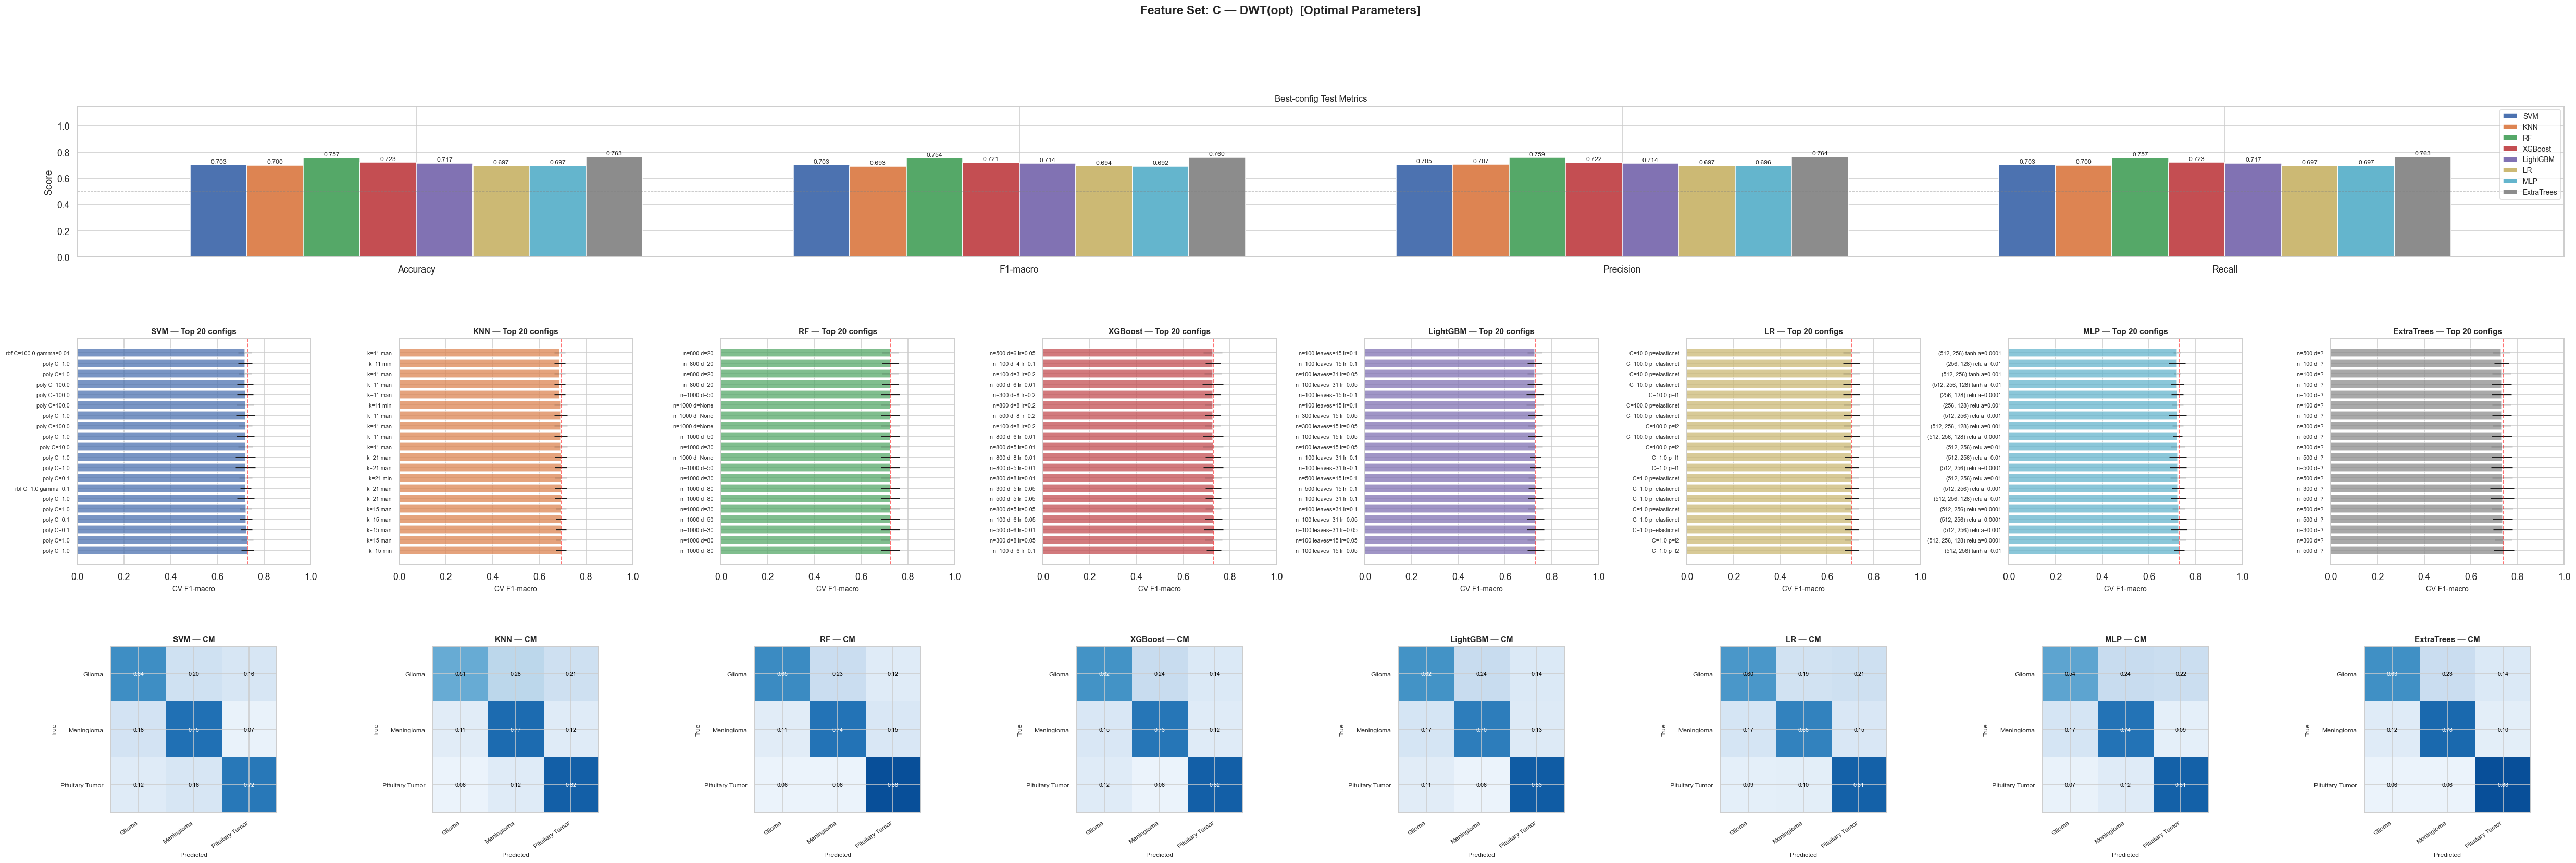
\includegraphics[width=\linewidth,height=0.30\textheight,keepaspectratio]{p2_C_—_DWT(opt).png}
    \column{0.48\textwidth}
    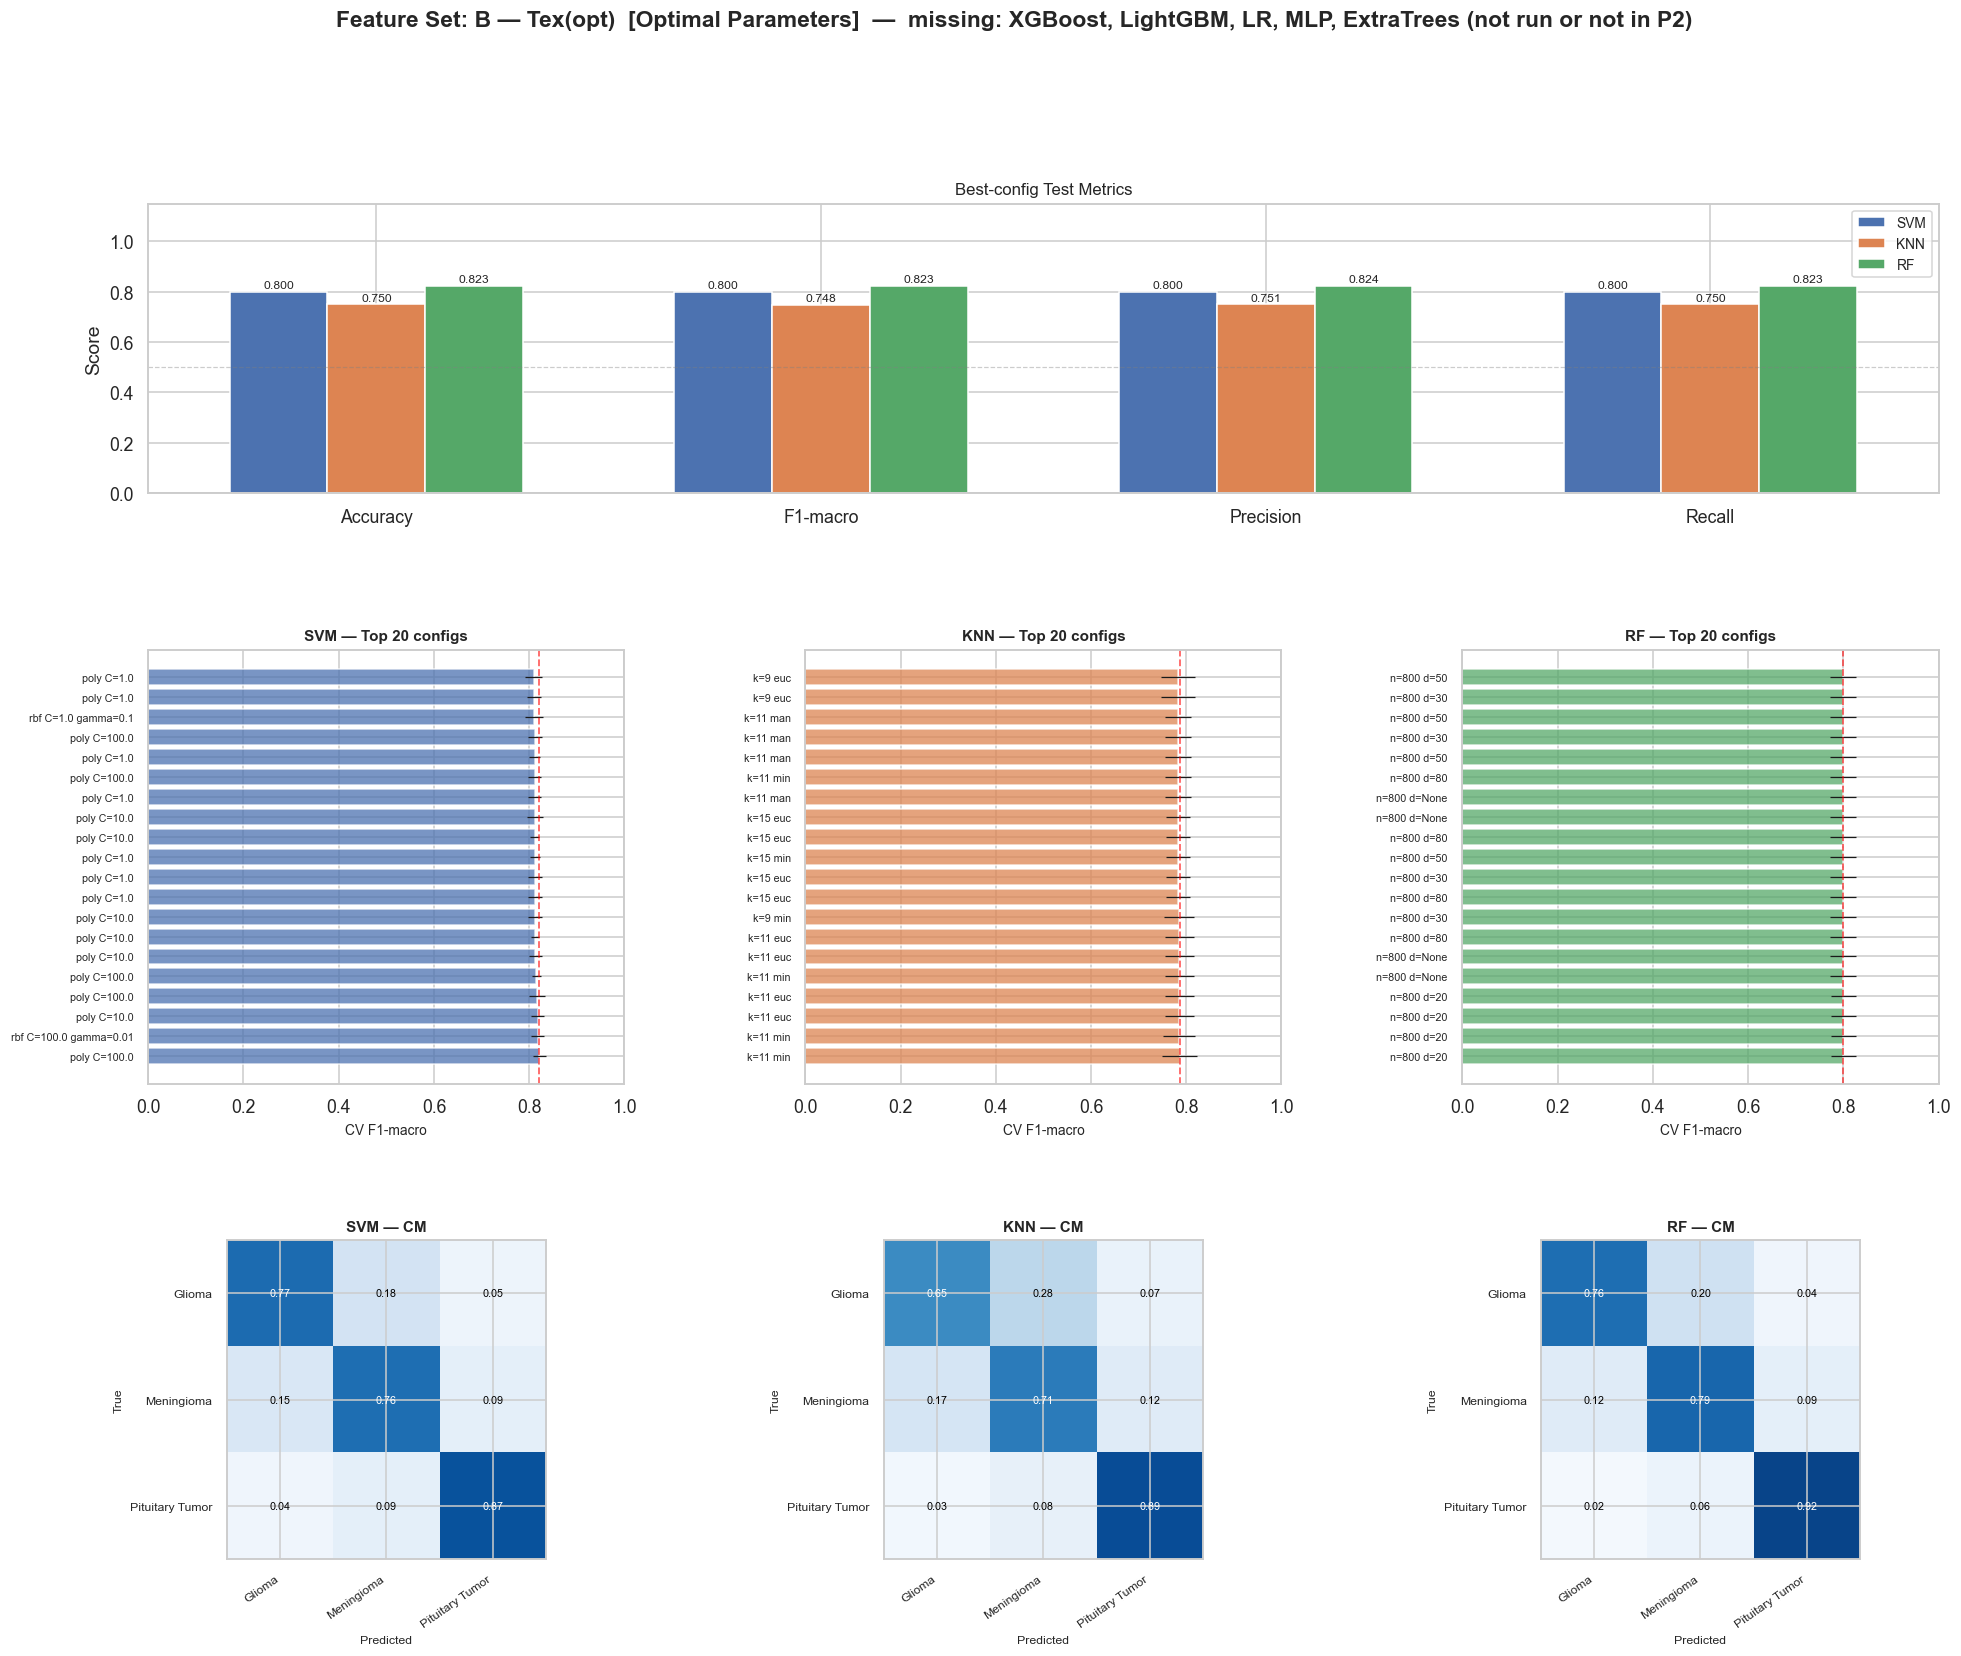
\includegraphics[width=\linewidth,height=0.30\textheight,keepaspectratio]{p2_B_—_Tex(opt).png}\\[0.1em]
    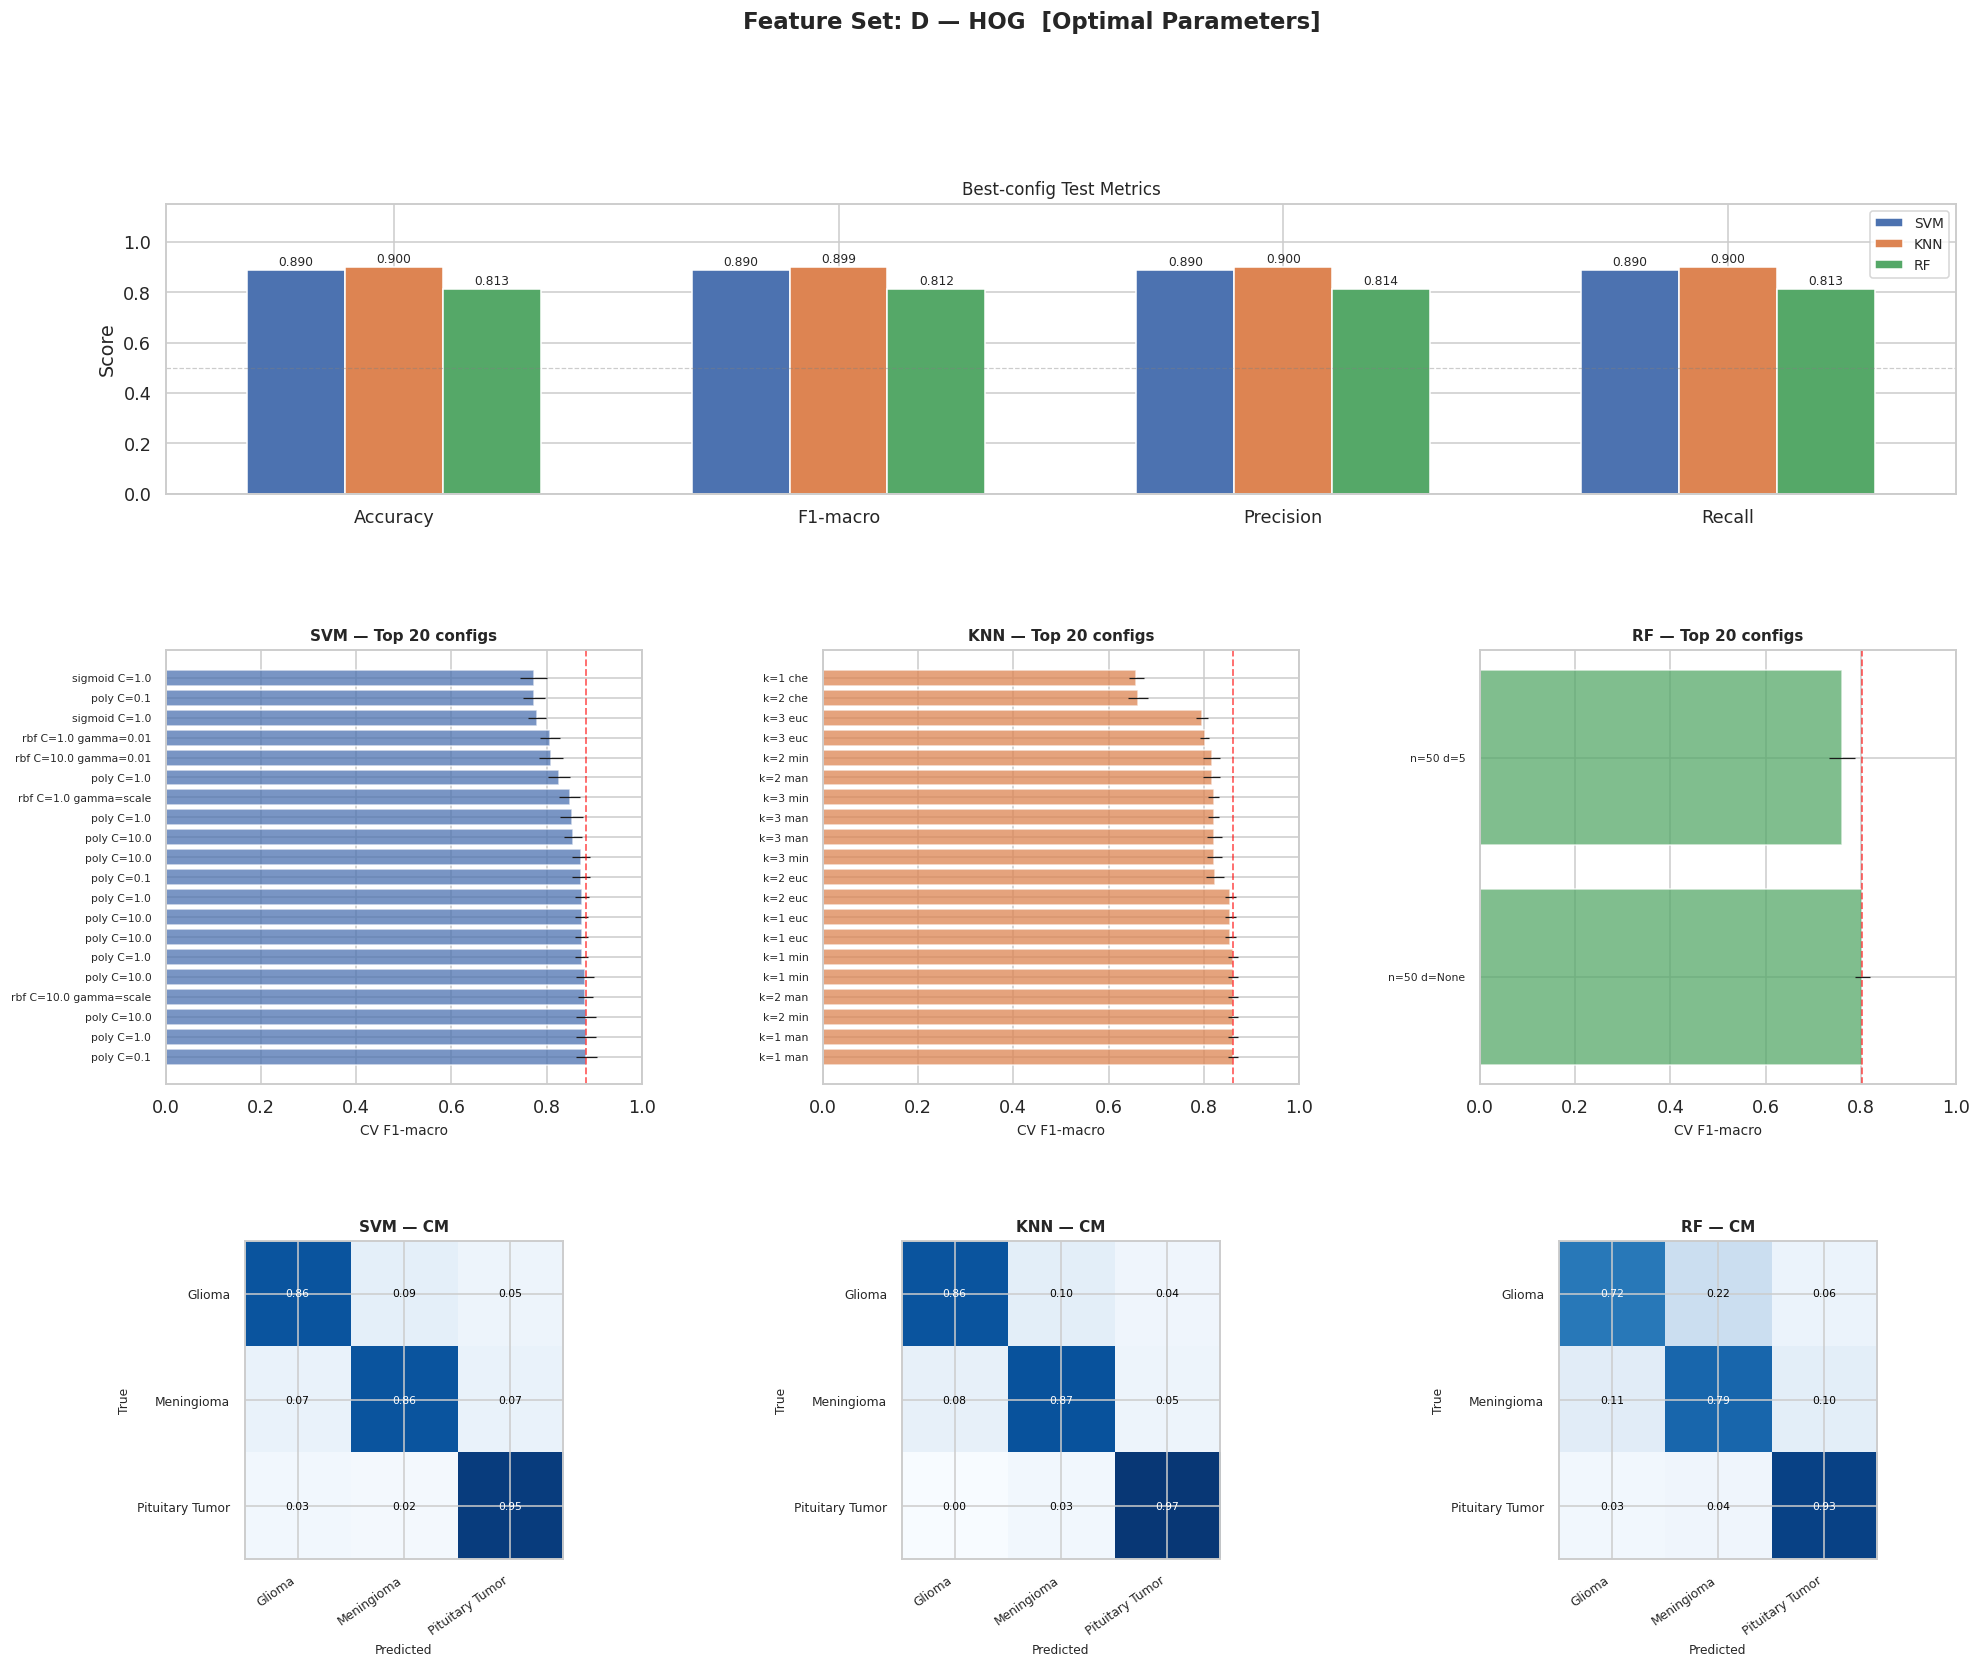
\includegraphics[width=\linewidth,height=0.30\textheight,keepaspectratio]{p2_D_—_HOG.png}
  \end{columns}
  \vspace{-0.3em}
  {\scriptsize \textbf{Best per branch:} A/SVM \AccAStats{} \quad B/XGB \AccBTex{} \quad C/RF \AccCDwt{} \quad D/SVM \AccDHog{}}
\end{frame}

\note{
HOG alone reaches 90.3\% --- strongest individual family.
Statistics and DWT are weaker alone but may contribute complementary signal when fused.
}

% Slide 17 — Combined Feature Results
\begin{frame}[shrink=8]{Combined Feature Results}
  \centering
  \begin{columns}[T,onlytextwidth]
    \column{0.48\textwidth}
    
\includegraphics[width=\linewidth,height=0.28\textheight,keepaspectratio]{p2_ApB.png}\\[0.1em]
    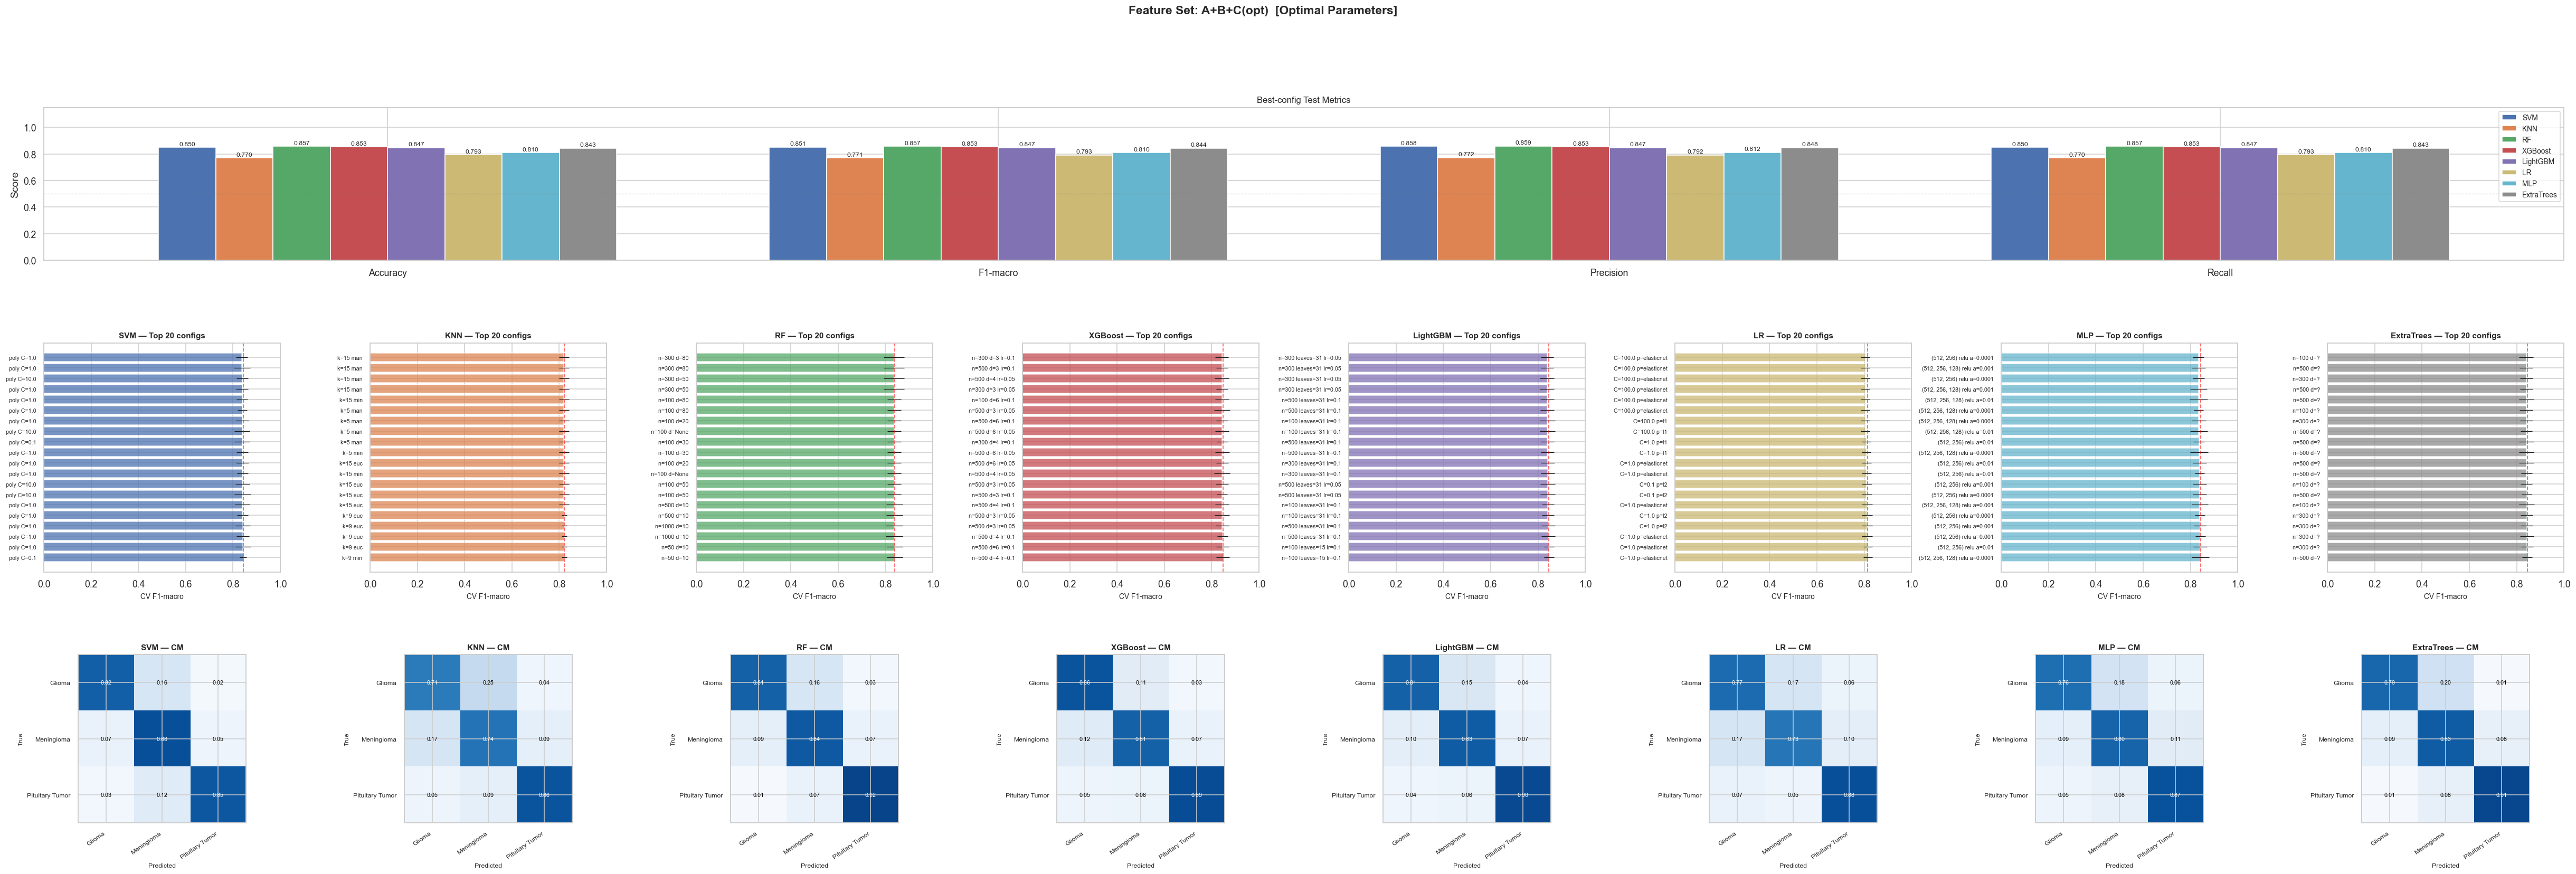
\includegraphics[width=\linewidth,height=0.28\textheight,keepaspectratio]{p2_ApBpC(opt).png}
    \column{0.48\textwidth}
    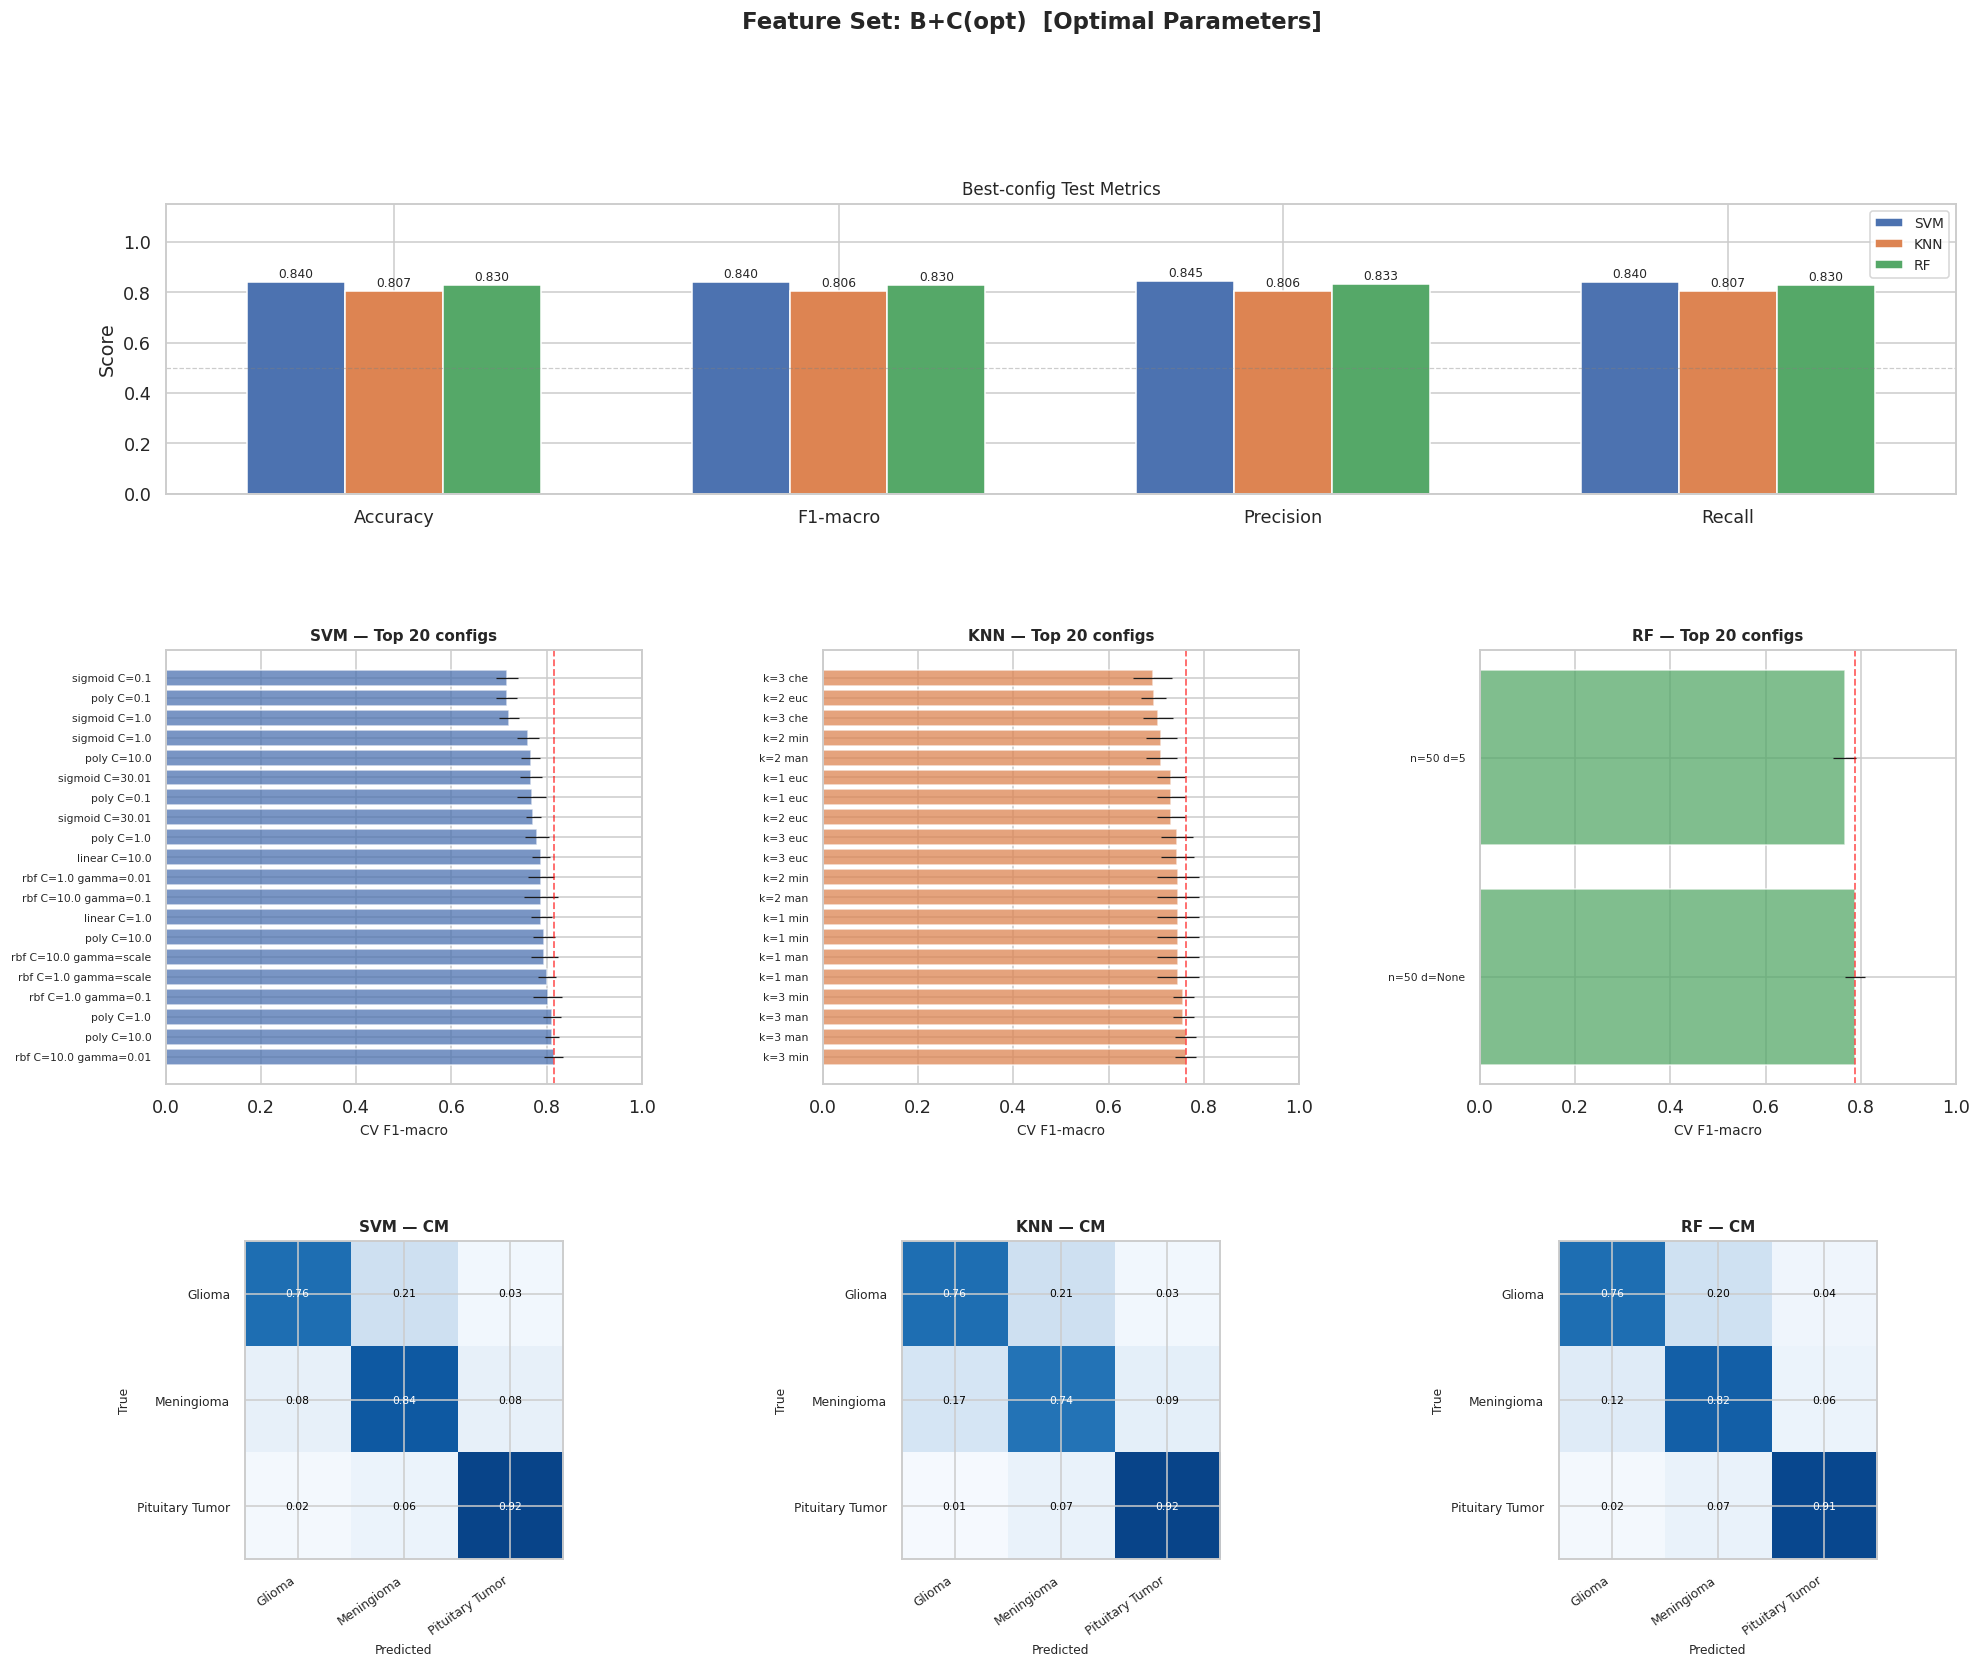
\includegraphics[width=\linewidth,height=0.28\textheight,keepaspectratio]{p2_BpC(opt).png}\\[0.1em]
    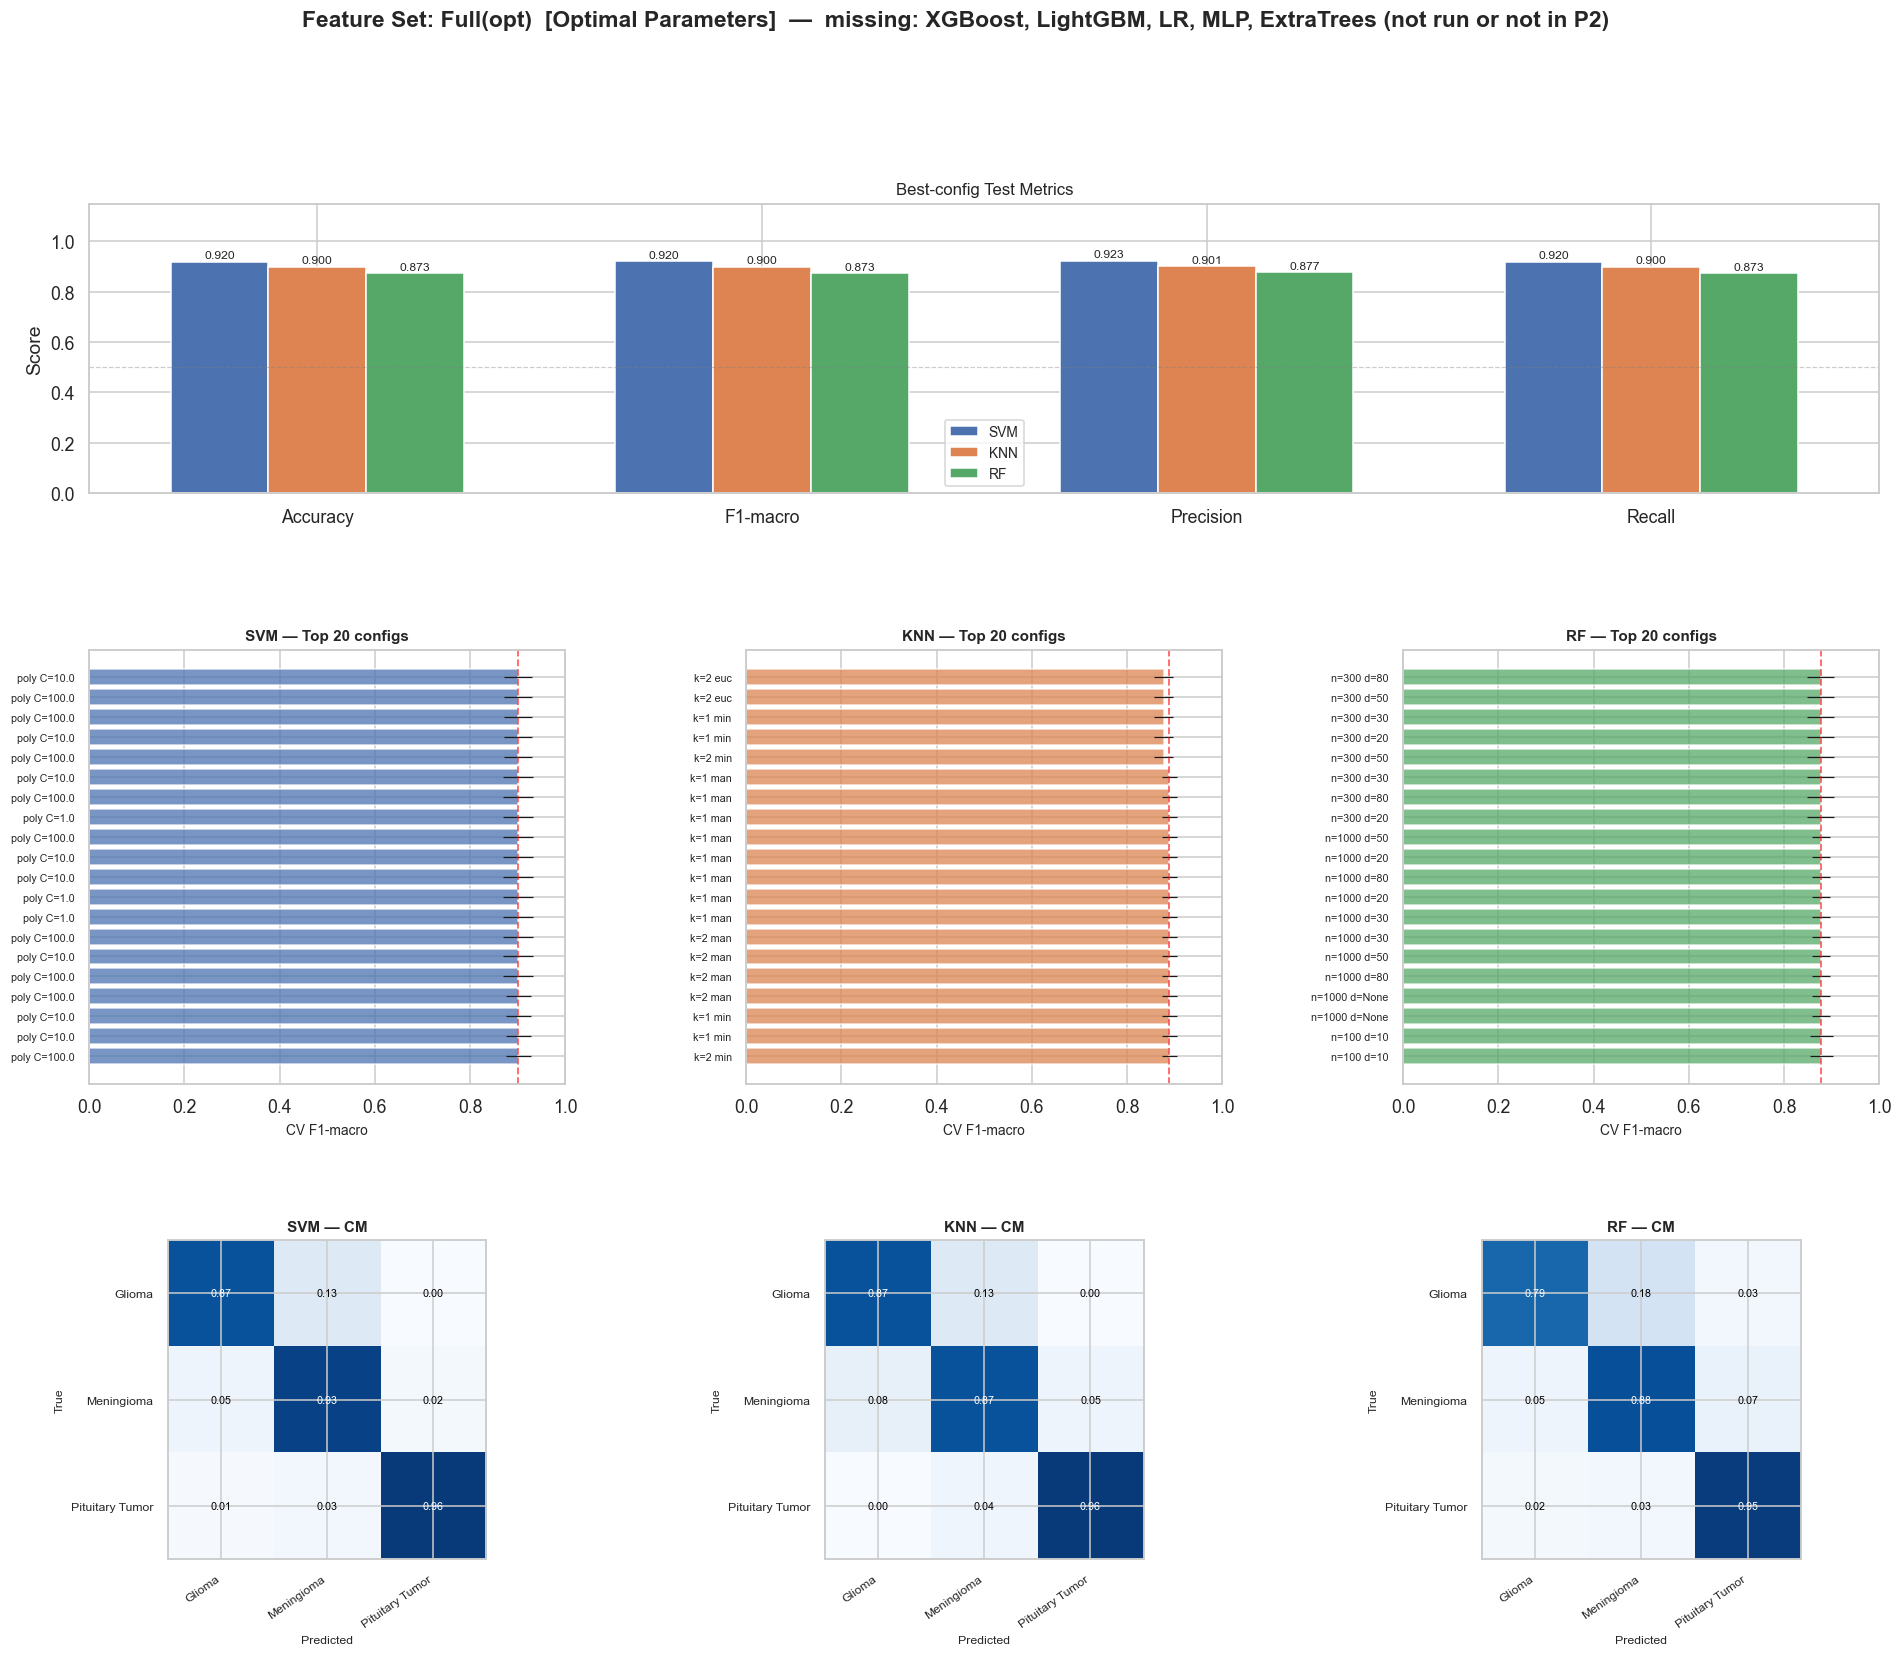
\includegraphics[width=\linewidth,height=0.28\textheight,keepaspectratio]{p2_Full(opt).png}
  \end{columns}
  \vspace{-0.2em}
  {\scriptsize Fusion improves performance: Full(opt) reaches \BestAcc{} (+ \FusionGain{} pp over HOG alone).}
\end{frame}

\note{
Fusion helps most when combined with kernel methods.
Full(opt)+SVM is the clear winner at 92\% accuracy.
}

% Slide 18 — Global Ranking
\begin{frame}[shrink=5]{Global Ranking}
  \begin{columns}[T,onlytextwidth]
    \column{0.42\textwidth}
    \begin{block}{Top 5 (held-out test)}
      \begin{table}
\centering
\footnotesize
\begin{tabular}{@{}clccc@{}}
\toprule
\textbf{Rank} & \textbf{Feature set / Model} & \textbf{F1-macro} & \textbf{Acc.} & \textbf{$\kappa$} \\
\midrule
1 & \textbf{Full(opt) / SVM} & \textbf{\BestFOne} & \textbf{\BestAcc} & \textbf{\BestKappa} \\
2 & D — HOG / SVM & \RankTwoFOne & \HogSvmAcc & 0.855 \\
3 & Full(opt) / KNN & \RankThreeFOne & 90.0\% & 0.85 \\
4 & D — HOG / KNN & \RankFourFOne & 89.7\% & 0.845 \\
5 & Full(opt) / LightGBM & \RankFiveFOne & 89.3\% & 0.84 \\
\bottomrule
\end{tabular}
\caption{Top 5 configurations (held-out test, ranked by F1-macro).}
\end{table}

    \end{block}

    \begin{block}{Key insight}
      \small \BestPipeline{} ranks first (macro-F1 \BestFOne).\vspace{0.2em}

      HOG+SVM is a strong single-family baseline, but fusion adds a consistent gain.
    \end{block}
    \column{0.56\textwidth}
    \centering
    
\includegraphics[width=\linewidth]{p2_leaderboard.png}
  \end{columns}
\end{frame}

\note{
Leaderboard ordered by F1-macro on held-out test.
Top 3 are all SVM or KNN on high-dimensional feature sets.
}

% Slide 19 — Feature Importance
\begin{frame}[shrink=2]{Feature Importance Analysis}
  \begin{columns}[T,onlytextwidth]
    \column{0.68\textwidth}
    \centering
    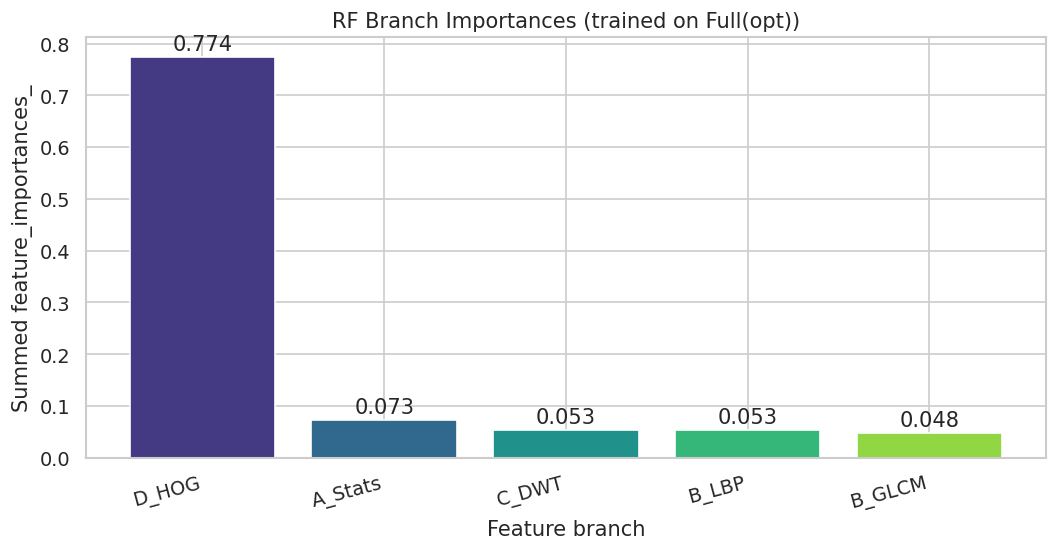
\includegraphics[width=\linewidth,height=0.66\textheight,keepaspectratio]{rf_branch_importance.png}

    \column{0.30\textwidth}
    \begin{block}{What this shows}
      \small We group Full(opt) features by descriptor family and estimate their relative influence
      using a Random Forest surrogate model.
    \end{block}

    \begin{block}{Takeaway}
      \small HOG and LBP dominate, while Stats and DWT provide smaller complementary gains.\vspace{0.2em}

      This matches the observed improvement from HOG $\rightarrow$ Full(opt).
    \end{block}
  \end{columns}
\end{frame}

\note{
Trained RF on Full(opt) features grouped by descriptor family.
HOG dominates due to high-dimensional edge information; LBP adds texture signal.
}

% Slide 20 — Feature Space Visualization
\begin{frame}[shrink=2]{Feature Space Visualization}
  \begin{columns}[T,onlytextwidth]
    \column{0.70\textwidth}
    \centering
    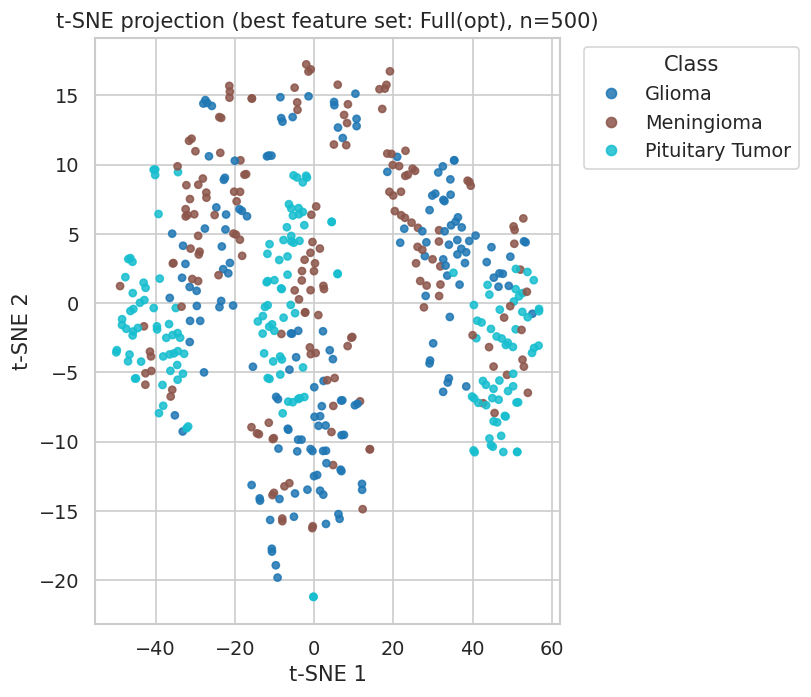
\includegraphics[width=\linewidth,height=0.70\textheight,keepaspectratio]{tsne_best_feature_set.png}

    \column{0.28\textwidth}
    \begin{block}{What is plotted}
      \small 2D t-SNE projection of 526-dimensional Full(opt) feature vectors.
    \end{block}

    \begin{block}{Interpretation}
      \small Partial separation indicates discriminative power.\vspace{0.2em}

      Glioma vs.\ meningioma overlap helps explain residual confusion even in the best model.
    \end{block}
  \end{columns}
\end{frame}

\note{
2D t-SNE projection of 526-dimensional Full(opt) features.
Good global structure but not perfect separation --- room for improvement.
}

% Slide 21 — Stability Analysis
\begin{frame}[shrink=2]{Stability Analysis}
  \begin{columns}[T,onlytextwidth]
    \column{0.50\textwidth}
    \begin{block}{Seed stability (Full(opt) + SVM)}
      \begin{table}
\centering
\footnotesize
\begin{tabular}{@{}cccc@{}}
\toprule
\textbf{Seed} & \textbf{Accuracy} & \textbf{F1-macro} \\
\midrule
42 & 0.9500 & 0.9498 \\
43 & 0.9100 & 0.9099 \\
44 & 0.9133 & 0.9130 \\
\midrule
\textbf{Mean $\pm$ CI} & --- & \textbf{\SeedFOneMean{} $\pm$ \SeedFOneCI} \\
\bottomrule
\end{tabular}
\caption{Seed stability for Full(opt) + SVM (re-split per seed).}
\end{table}

    \end{block}

    \column{0.48\textwidth}
    \begin{block}{Setup}
      \small Three independent train/test splits (seeds 42, 43, 44).\vspace{0.2em}

      Hyperparameters are re-tuned per seed (same protocol, different partition).
    \end{block}

    \begin{block}{Quick visual (F1-macro)}
      \centering
      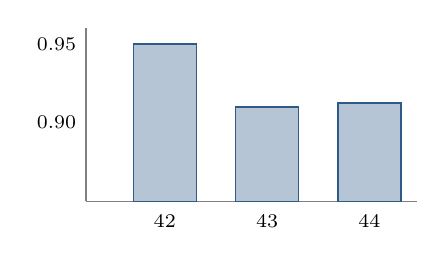
\begin{tikzpicture}[x=1cm,y=1cm]
        \draw[gray] (0,0) -- (4.2,0);
        \draw[gray] (0,0) -- (0,2.2);
        \node[anchor=east] at (0,2.0) {\scriptsize 0.95};
        \node[anchor=east] at (0,1.0) {\scriptsize 0.90};
        \draw[fill=accent!35,draw=accent] (0.6,0) rectangle (1.4,2.0);
        \draw[fill=accent!35,draw=accent] (1.9,0) rectangle (2.7,1.2);
        \draw[fill=accent!35,draw=accent] (3.2,0) rectangle (4.0,1.25);
        \node at (1.0,-0.25) {\scriptsize 42};
        \node at (2.3,-0.25) {\scriptsize 43};
        \node at (3.6,-0.25) {\scriptsize 44};
      \end{tikzpicture}
    \end{block}

    \begin{block}{Conclusion}
      \small Mean macro-F1: \keyresult{\SeedFOneMean{} $\pm$ \SeedFOneCI}.\;
      Low variation suggests the pipeline is not dependent on a single split.
    \end{block}
  \end{columns}
\end{frame}

\note{
Seed 42 yields highest score due to favorable test partition.
Mean F1 across seeds remains above 0.91.
}

% Slide 22 — Statistical Validation
\begin{frame}[shrink=2]{Statistical Validation}
  \begin{columns}[T,onlytextwidth]
    \column{0.33\textwidth}
    \begin{block}{Cross-validation (5-fold)}
      \small
      \begin{tabular}{@{}ll@{}}
        \toprule
        F1-macro & \BestFOneCVMean{} $\pm$ \BestFOneCVStd{} \\
        Accuracy & \BestAccCVMean{} $\pm$ \BestAccCVStd{} \\
        \bottomrule
      \end{tabular}

      \vspace{0.2em}
      {\scriptsize Stable performance across folds supports generalization.}
    \end{block}

    \column{0.33\textwidth}
    \begin{block}{Bootstrap CI (95\%, test)}
      \small
      \begin{tabular}{@{}ll@{}}
        \toprule
        F1-macro & [\BestFOneCILow,\; \BestFOneCIHigh] \\
        Accuracy & [\BestAccCILow,\; \BestAccCIHigh] \\
        \bottomrule
      \end{tabular}

      \vspace{0.2em}
      {\scriptsize Uncertainty bounds on the held-out test estimate.}
    \end{block}

    \column{0.33\textwidth}
    \begin{block}{Significance tests}
      \small
      \begin{tabular}{@{}p{0.55\linewidth}p{0.35\linewidth}@{}}
        \toprule
        \textbf{Test} & \textbf{Result} \\
        \midrule
        McNemar (SVM vs RF) & $p{=}$\McNemarRF \\
        McNemar (SVM vs XGB) & $p{=}$\McNemarXGB \\
        McNemar (SVM vs KNN) & $p{=}$\McNemarKNN \\
        Friedman (within Full) & $p{=}$\FriedmanFullP \\
        \bottomrule
      \end{tabular}

      \vspace{0.2em}
      {\scriptsize Confirms SVM improvements are meaningful vs several baselines.}
    \end{block}
  \end{columns}
\end{frame}

\note{
Multiple validation layers confirm improvements are meaningful, not random.
SVM advantage over tree ensembles is statistically supported.
}

% Slide 23 — Best Model (key result)
\begin{frame}[shrink=2]{Best Model}
  \begin{columns}[T,onlytextwidth]
    \column{0.42\textwidth}
    \begin{block}{Final pipeline}
      \centering
      {\Large \BestPipeline}
      \vspace{0.4em}

      
\begin{tikzpicture}[
        node distance=0.45cm,
        box/.style={rectangle, rounded corners=2pt, draw=accent, fill=lightbg,
                    minimum height=0.7cm, minimum width=0.92\linewidth, align=center, font=\small},
        arr/.style={-{Stealth[length=2mm]}, thick, accent}
      ]
        \node[box] (fs) {Full(opt) features\\(526 cleaned)};
        \node[box, below=of fs] (svm) {SVM (poly kernel)};
        \node[box, below=of svm] (pred) {3-class prediction};
        \draw[arr] (fs) -- (svm);
        \draw[arr] (svm) -- (pred);
      \end{tikzpicture}
    \end{block}

    \begin{block}{Uncertainty}
      \small 95\% bootstrap CI (macro-F1): [\BestFOneCILow,\; \BestFOneCIHigh]
    \end{block}

    \column{0.56\textwidth}
    \begin{block}{Performance (held-out test)}
      \small
      \begin{tabular}{@{}ll@{}}
        \toprule
        \textbf{Metric} & \textbf{Value} \\
        \midrule
        Accuracy & \keyresult{\BestAcc} \\
        Precision (macro) & \BestPrecision \\
        Recall (macro) & \BestRecall \\
        F1-macro & \keyresult{\BestFOne} \\
        Cohen's $\kappa$ & \BestKappa \\
        \bottomrule
      \end{tabular}
    \end{block}
  \end{columns}
\end{frame}

\note{
This is the key result slide. Full(opt)+SVM achieves 92\% accuracy with strong
per-class balance. Emphasize this is traditional ML on a modest dataset.
}

% Slide 24 — Discussion
\begin{frame}[shrink=2]{Discussion}
  \begin{columns}[T,onlytextwidth]
    \column{0.58\textwidth}
    \begin{block}{Why optimization + fusion help}
      \small Phase 1 ranks descriptor parameters using separability metrics, reducing
      trial-and-error in Phase 2.\vspace{0.2em}

      Fusion combines complementary cues: intensity (A), texture (B), frequency (C), and edges (D).
    \end{block}

    \begin{block}{Why SVM performs best here}
      \small The polynomial kernel captures non-linear interactions in the 526-D Full(opt) space.\vspace{0.2em}

      High-dimensional HOG features often favor margin-based learning over bagging-style ensembles.
    \end{block}

    \begin{block}{Practical implications}
      \small CPU-only, reproducible, and descriptor-based interpretability.\vspace{0.2em}

      The goal is decision support; clinical deployment requires external validation and workflow integration.
    \end{block}

    \column{0.40\textwidth}
    \centering
    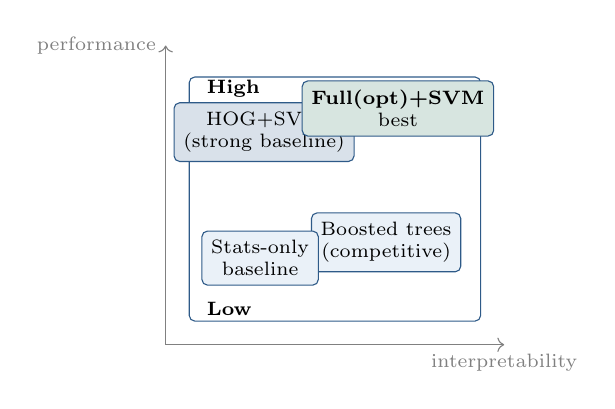
\begin{tikzpicture}[x=1cm,y=1cm]
      \draw[->,gray] (0,0) -- (4.3,0) node[below] {\scriptsize interpretability};
      \draw[->,gray] (0,0) -- (0,3.8) node[left] {\scriptsize performance};

      \draw[draw=accent,rounded corners=2pt] (0.3,0.3) rectangle (4.0,3.4);
      \node[anchor=west] at (0.4,3.25) {\scriptsize \textbf{High}};
      \node[anchor=west] at (0.4,0.45) {\scriptsize \textbf{Low}};

      \node[draw=accent,fill=accent!18,rounded corners=2pt,align=center,font=\scriptsize] at (1.25,2.7) {HOG+SVM\\(strong baseline)};
      \node[draw=accent,fill=accent2!18,rounded corners=2pt,align=center,font=\scriptsize] at (2.95,3.0) {\textbf{Full(opt)+SVM}\\best};
      \node[draw=accent,fill=lightbg,rounded corners=2pt,align=center,font=\scriptsize] at (2.8,1.3) {Boosted trees\\(competitive)};
      \node[draw=accent,fill=lightbg,rounded corners=2pt,align=center,font=\scriptsize] at (1.2,1.1) {Stats-only\\baseline};
    \end{tikzpicture}

    \vspace{0.2em}
    {\scriptsize Trade-off sketch (relative positioning).}
  \end{columns}
\end{frame}

\note{
Discuss trade-offs honestly. 92\% is strong for traditional ML but DL methods
may exceed this with more data. Our pipeline is transparent and reproducible.
}

% Slide 25 — Conclusion and Future Work
\begin{frame}[shrink=2]{Conclusion and Future Work}
  \begin{columns}[T,onlytextwidth]
    \column{0.56\textwidth}
    \begin{block}{Main contributions}
      \small
      \begin{tabular}{@{}p{0.35\linewidth}p{0.60\linewidth}@{}}
        \toprule
        \textbf{Contribution} & \textbf{Outcome} \\
        \midrule
        Feature optimization & separability-driven parameter selection \\
        Benchmarking & \NModels{} models $\times$ \NFeatureSets{} feature sets \\
        Validation & CV + bootstrap CI + significance tests \\
        Best pipeline & \BestPipeline{} at \keyresult{\BestAcc} \\
        \bottomrule
      \end{tabular}
    \end{block}

    \begin{block}{Final takeaway}
      \small \keyresult{Optimized handcrafted features + classical ML can be strong on modest MRI datasets}
      while remaining transparent and CPU-friendly.
    \end{block}

    \column{0.40\textwidth}
    \begin{block}{Future work roadmap}
      \centering
      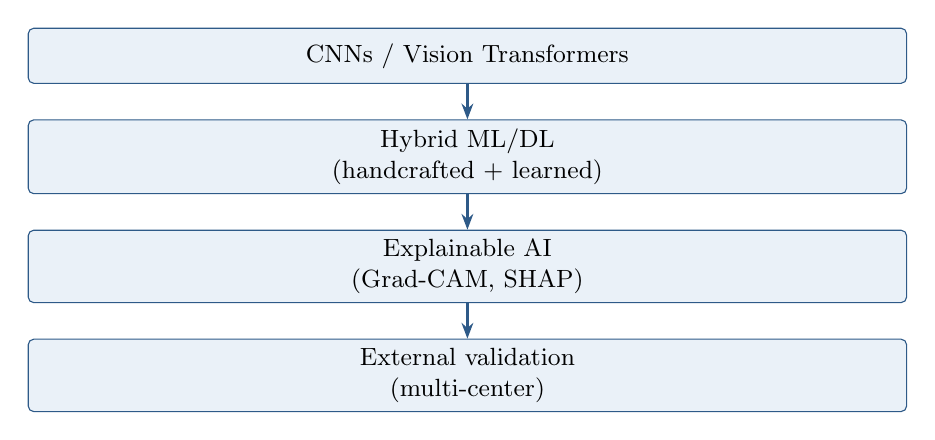
\begin{tikzpicture}[
        node distance=0.45cm,
        box/.style={rectangle, rounded corners=2pt, draw=accent, fill=lightbg,
                    minimum height=0.7cm, minimum width=0.92\linewidth, align=center, font=\small},
        arr/.style={-{Stealth[length=2mm]}, thick, accent}
      ]
        \node[box] (dl) {CNNs / Vision Transformers};
        \node[box, below=of dl] (hyb) {Hybrid ML/DL\\(handcrafted + learned)};
        \node[box, below=of hyb] (xai) {Explainable AI\\(Grad-CAM, SHAP)};
        \node[box, below=of xai] (ext) {External validation\\(multi-center)};
        \draw[arr] (dl) -- (hyb);
        \draw[arr] (hyb) -- (xai);
        \draw[arr] (xai) -- (ext);
      \end{tikzpicture}
    \end{block}
  \end{columns}
\end{frame}

\note{
Thank the audience. Key takeaway: careful feature engineering still competes with
deep learning on modest datasets. Open for questions.
}


\end{document}
